%-*- coding: UTF-8 -*-
% notes.tex
%
\documentclass[UTF8]{article}
\usepackage{geometry}
\geometry{a4paper, centering, scale=0.8}
\usepackage{minted}
\usepackage{hyperref}
\usepackage{indentfirst}    % to indent the first paragraph of a section
\usepackage{graphicx}       % to insert figures
\usepackage{amsmath}        % to type some math equations
\usepackage{amssymb}        % to use some special math font
\usepackage{IEEEtrantools}  % to use IEEEeqnarray
\usepackage{ulem}           % to use stikeout command \sout{} (don't work in math mode)
\usepackage{algorithm2e}    % to use algorithm environment
\usepackage{multicol}       % to display some content in multi-columns
\setlength{\columnseprule}{0.4pt}   % set the rule's width of multicols
\setlength{\columnsep}{5em}         % set the sep of multicols

% Math notation
% refered to https://github.com/exacity/deeplearningbook-chinese/blob/master/math_symbol.tex
\newcommand{\Scalar}[1]{\mathit{#1}}                % Scalar, the default math font
\newcommand{\Vector}[1]{\boldsymbol{\mathit{#1}}}   % Vector
\newcommand{\Matrix}[1]{\boldsymbol{\mathit{#1}}}   % Matrix
\newcommand{\Tensor}[1]{\textsf{\textbf{#1}}}       % Tensor
\newcommand{\Set}[1]{\mathbb{#1}}                   % Set
\newcommand{\Cal}[1]{\mathcal{#1}}                  % Math Cal

% Draw the lines in a matrix, which is composed by a series of vectors
\newcommand{\vRule}{\rule{0.3pt}{10mm}}             % vertical rule
\newcommand{\hRule}{\,\rule[1mm]{10mm}{0.3pt}\,}    % horizontal rule

\title{Deep Learning Specialization \\
        Neural Networks and Deep Learning \\
        Learning Notes}
\author{Du Ang \\ \texttt{du2ang233@gmail.com} }
\date{\today}

\begin{document}
\maketitle

\tableofcontents
\newpage

\section{Welcome}
\begin{quote}
    \emph{AI is the new Electricity. --- Andrew Ng}
\end{quote}

Electricity had once transformed countless industries: transportation, manufacturing, healthcare,
communications, and more.

AI will now bring about an equally big transformation.

\paragraph{Courses in this sequence (Specialization):}
\begin{enumerate}
    \item \emph{Neural Networks and Deep Learning}
    \item \emph{Improving Deep Neural Networks: Hyperparameter tuning, Regularization and
    Optimization}
    \item \emph{Structuring Machine Learning Projects}
    \item \emph{Convolutional Neural Networks}
    \item \emph{Sequence Models}
\end{enumerate}

\section{Introduction to Deep Learning}
\subsection{What is a neural network?}
It is powerful learning algorithm inspired by how the brain works.
\subsubsection{Single neural network}
Given data about the size of houses on the real estate market and you want to fit a function that
will predict their price. It is a linear regression problem because the price as a function of size
is a continuous output.

We know the prices can never be negative so we are creating a function called Rectified Linear Unit
(ReLU) which starts at zero.
\begin{figure}[htb]
    \centering
    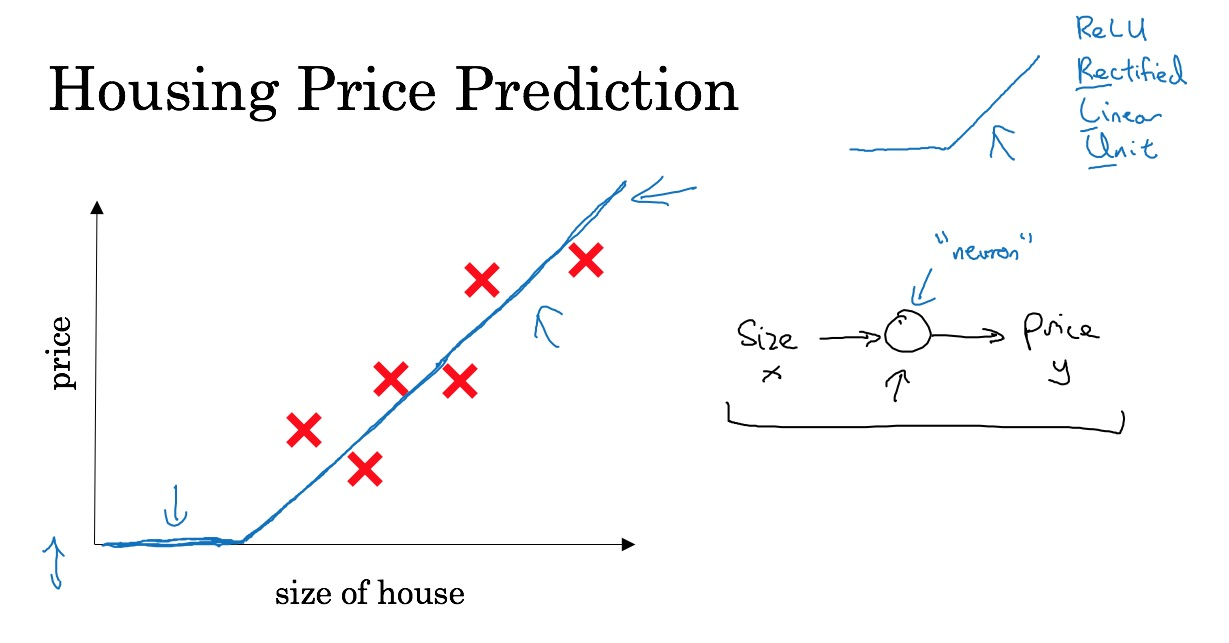
\includegraphics[width=40em]{figures/single-nn}
    \caption{The ``Housing Price Prediction'' problem. The input is the size of the house
    ($x$); The output is the price ($y$); The ``neuron'' implements the function
    ReLU.}
\end{figure}

\subsubsection{Multiple neural network}
The price of a house can be affected by other features such as size, number of bedrooms, zip code
and wealth. The role of the neural network is to predicted the price and it will automatically
generate the hidden units. We only need to give the inputs x and the output y.
\begin{figure}[htb]
    \centering
    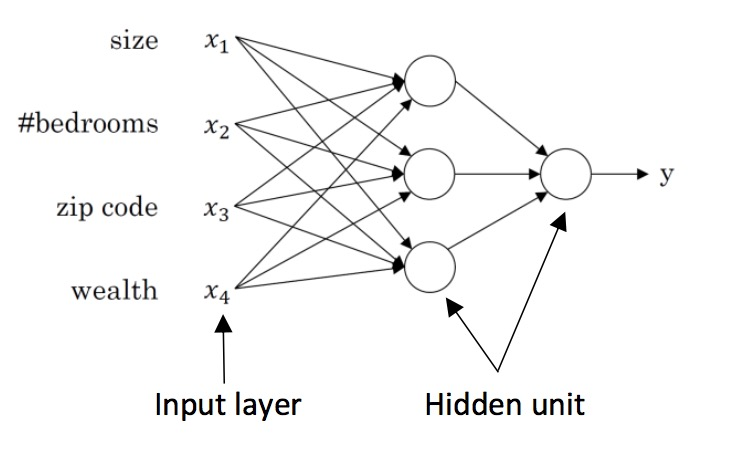
\includegraphics[width=30em]{figures/multiple-nn}
    \caption{Multiple neural network}
\end{figure}

\subsection{Supervised Learning}
In supervised learning, we are given a data set and already know about what our correct output
should look like, having the idea that there is a relationship between the input and the output.

Supervised learning problems are categorized into ``regression'' and ``classification'' problems.
In a regression problem, we are trying to predict results with a continuous output, meaning that we
are trying to map input variables to some continuous function. In a classification problem, we are
instead trying to predict results in a discrete output. In other words, we are trying to map input
variables into discrete categories.

Here are some example of supervised learning:
\begin{table}[htb]
\centering
\caption{Supervised Learning Applications}
\begin{tabular}{lllc}
\textbf{Input($x$)} & \textbf{Output($y$)} & \textbf{Application}
& \textbf{NN Types} \\ \hline
Home features & Price & Real Estate & Standard NN \\
Ad, user info & Click on ad? (0/1) & Online Advertising & Standard NN \\
Image & Object (1, ..., 1000) & Photo tagging & CNN \\
Audio & Text transcript & Speech Recognition & RNN \\
English & Chinese & Machine translation & RNN \\
Image, Radar info & Position of other cars & Autonomous driving & Custom/Hybrid \\
\end{tabular}
\end{table}

There are different types of neural network, for example, Convolutional Neural Network (CNN) used
often for image application and Recurrent Neural Network (RNN) used for one-dimensional sequence
data such as translating English to Chinese or a temporal component such as text transcript. As for
the autonomous driving, it is a hybrid neural network architecture.

\subsubsection{Structured vs unstructed data}
Structed data refers to things that has a defined meaning such as price, age whereas unstructed
data refers to thing like pixel, raw audio, text.

\subsection{Why is Deep Learning taking off?}
Deep learning is taking off due to a large amount of data available through the digitization of the
society, faster computation and innovation in the development of neural network algorithm.
\begin{figure}[htb]
    \centering
    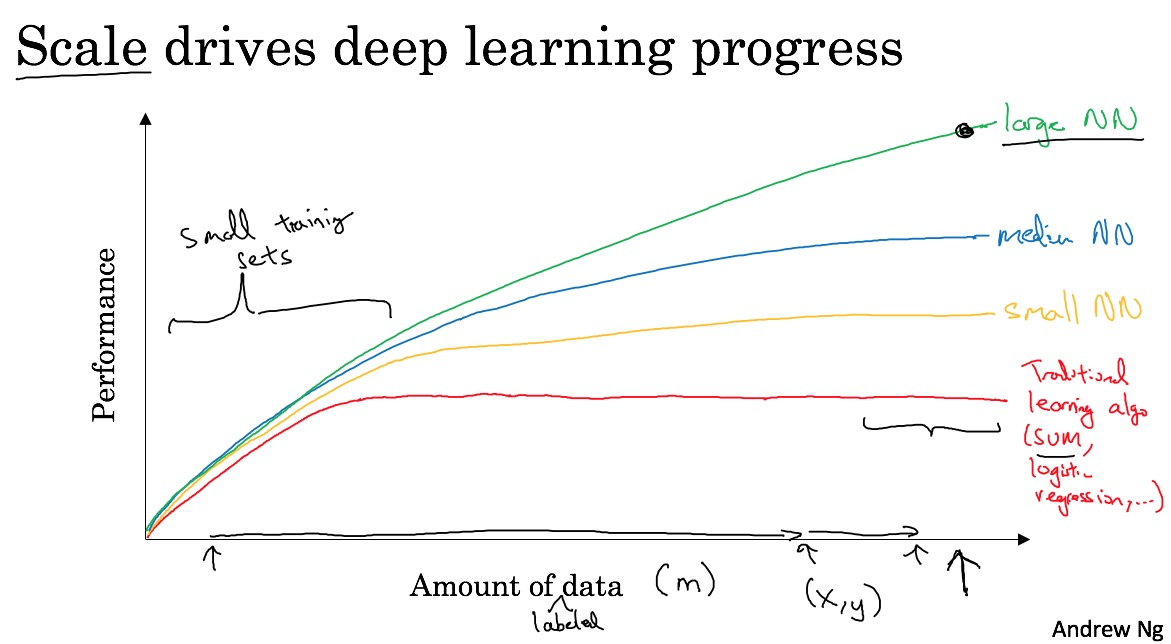
\includegraphics[width=40em]{figures/deep-nn-scale}
    \caption{Scale drives deep learning progress}
\end{figure}

Two things have to be considered to get to the high level of performance:
\begin{enumerate}
    \item Being able to train a big enough neural network
    \item Huge amount of labelled data
\end{enumerate}

The process of training a neural network is iterative:
\begin{figure}[htb]
    \centering
    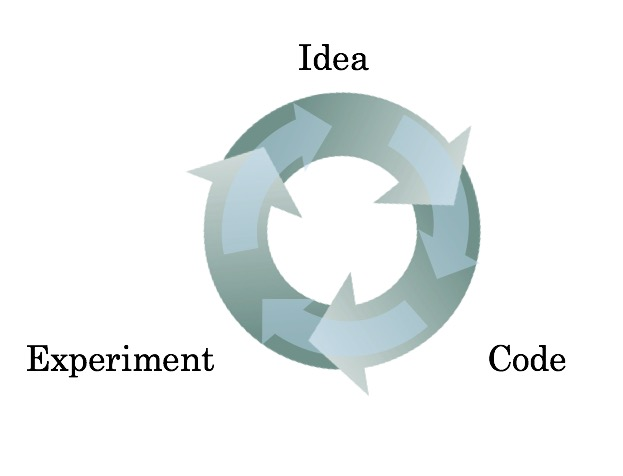
\includegraphics[width=25em]{figures/train-nn-process}
\end{figure}

It could take a good amount of time to train a neural network, which affects your productivity.
Faster computation helps to iterate and improve new algorithm.

\section{Neural Network Basics}
\subsection{Logistic Regression as a Neural Network}
\subsubsection{Binary Classification}
In a binary classification problem, the result is a discrete value output. For example:
\begin{itemize}
    \item account hacked (1) or compromised (0)
    \item a tumor malign (1) or benign (0)
\end{itemize}

\paragraph{Example: Cat vs Non-Cat}
The goal is to train a classifier that the input is an image represented by a feature vector,
$x$, and predicts whether the corresponding label $y$ is 1 or 0. In this case,
whether this is a cat image (1) or a non-cat image (0).

\begin{figure}[htb]
    \centering
    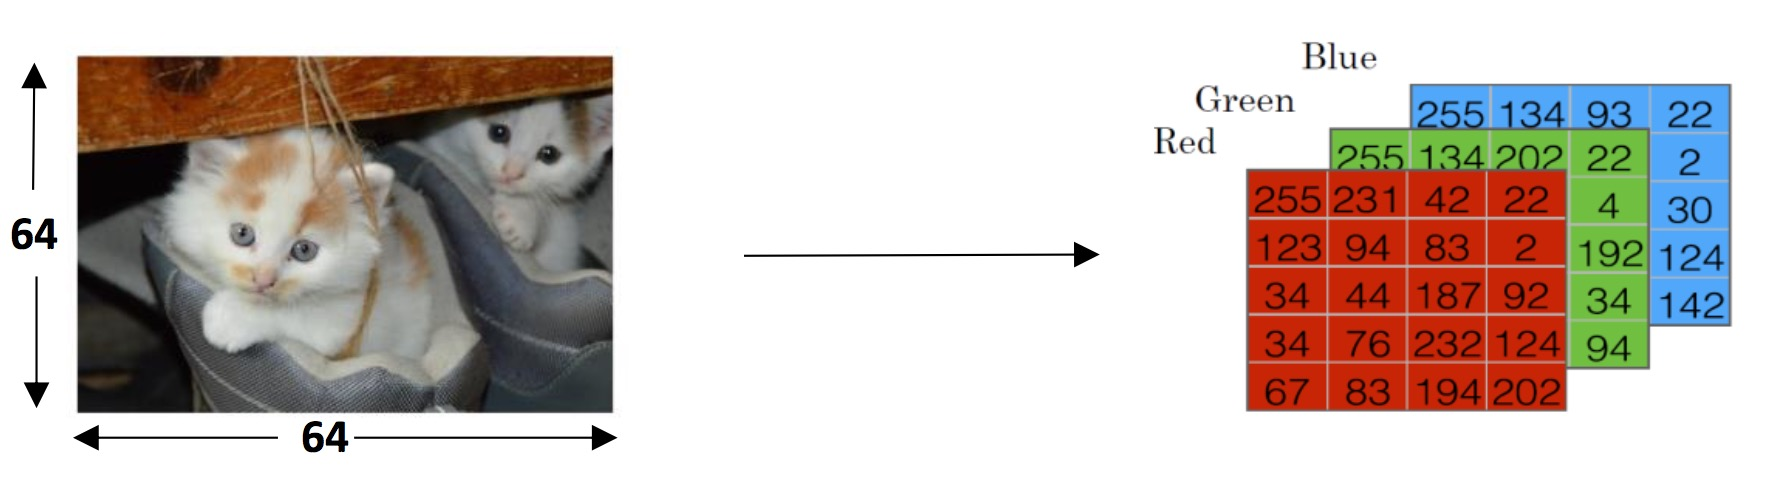
\includegraphics[width=35em]{figures/cat}
\end{figure}
An image is store in the computer in three separate matrices corresponding to the Red, Green, and
Blue color channels of the image. The three matrices have the same size as the image, for example,
the resolution of the cat image is 64 pixels $\times$ 64 pixels, the three matrices (RGB) are 64
$\times$ 64 each.

The value in a cell represents the pixel intensity which will be used to create a feature vector of
n-dimension. In pattern recognition and machine learning, a feature vector represents an object, in
this case, a cat or no cat.

To create a feature vector, $\Vector{x}$, the pixel intensity values will be ``unroll'' or
``reshape'' for each color. The dimension of the input feature vector $\Vector{x}$, is
$n_x = 64 \times 64 \times 3 = 12288$.
\begin{figure}[htb]
    \centering
    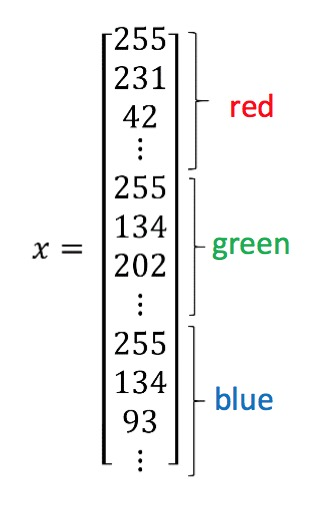
\includegraphics[width=10em]{figures/unrolled-image}
\end{figure}

\subsubsection{Notation}
single example: $(\Vector{x}, y)$, $\Vector{x} \in \Set{R}^{n_x}$, $y \in \{0, 1\}$

$m$ training examples: $\{(\Vector{x}^{(1)}, y^{(2)}), (\Vector{x}^{(2)}, y^{(2)}), \ldots,
(\Vector{x}^{(m)}, y^{(m)})\}$

$m = m_{train}$ \qquad $m_{test}$ = the number of test examples

\begin{IEEEeqnarray*}{rCl}
    \Matrix{X} = \left[
        \begin{array}{cccc}
            \vRule & \vRule & & \vRule \\
            \Vector{x^{(1)}} & \Vector{x^{(2)}} & \cdots & \Vector{x^{(m)}} \\
            \vRule & \vRule & & \vRule
        \end{array}
    \right]
    \qquad
    \Matrix{X} \in \Set{R}^{{n_x} \times m}
\end{IEEEeqnarray*}

\begin{IEEEeqnarray*}{rCl}
    \Vector{Y} = \left[
        \begin{array}{cccc}
            y^{(1)} & y^{(2)} & \cdots & y^{(m)}
        \end{array}
    \right]
    \qquad
    \Vector{Y} \in \Set{R}^{1 \times m}
\end{IEEEeqnarray*}

In Python/NumPy, \mintinline{numpy}{X.shape = (n_x, m), Y.shape = (1, m)}.

\subsubsection{Logistic Regression}
Logistic regression is a learning algorithm used in a supervised learning problem when the output
$y$ are all either zero or one. The goal of logistic regression is to minimize the error between
its predictions and training data.

\paragraph{Example: Cat vs Non-Cat}
Given an image represented by a feature vector $\Vector{x}$, the algorithm will evaluate the
probabilty of a cat being in that image.

Given $\Vector{x}$, want $\hat{y} = P(y=1|\Vector{x})$, $\Vector{x} \in \Set{R}^{n_x}$, $0 \leq
\hat{y} \leq 1$

Parameters: $\Vector{w} \in \Set{R}^{n_x}$, $b \in \Set{R}$

Output: \sout{$\hat{y} = \Vector{w}^T \Vector{x} + b$} \quad
$\hat{y} = \sigma (\Vector{w}^T\Vector{x} + b)$, where $\sigma(z) = \frac{1}{1+e^{-z}}$.
\begin{figure}[htb]
    \centering
    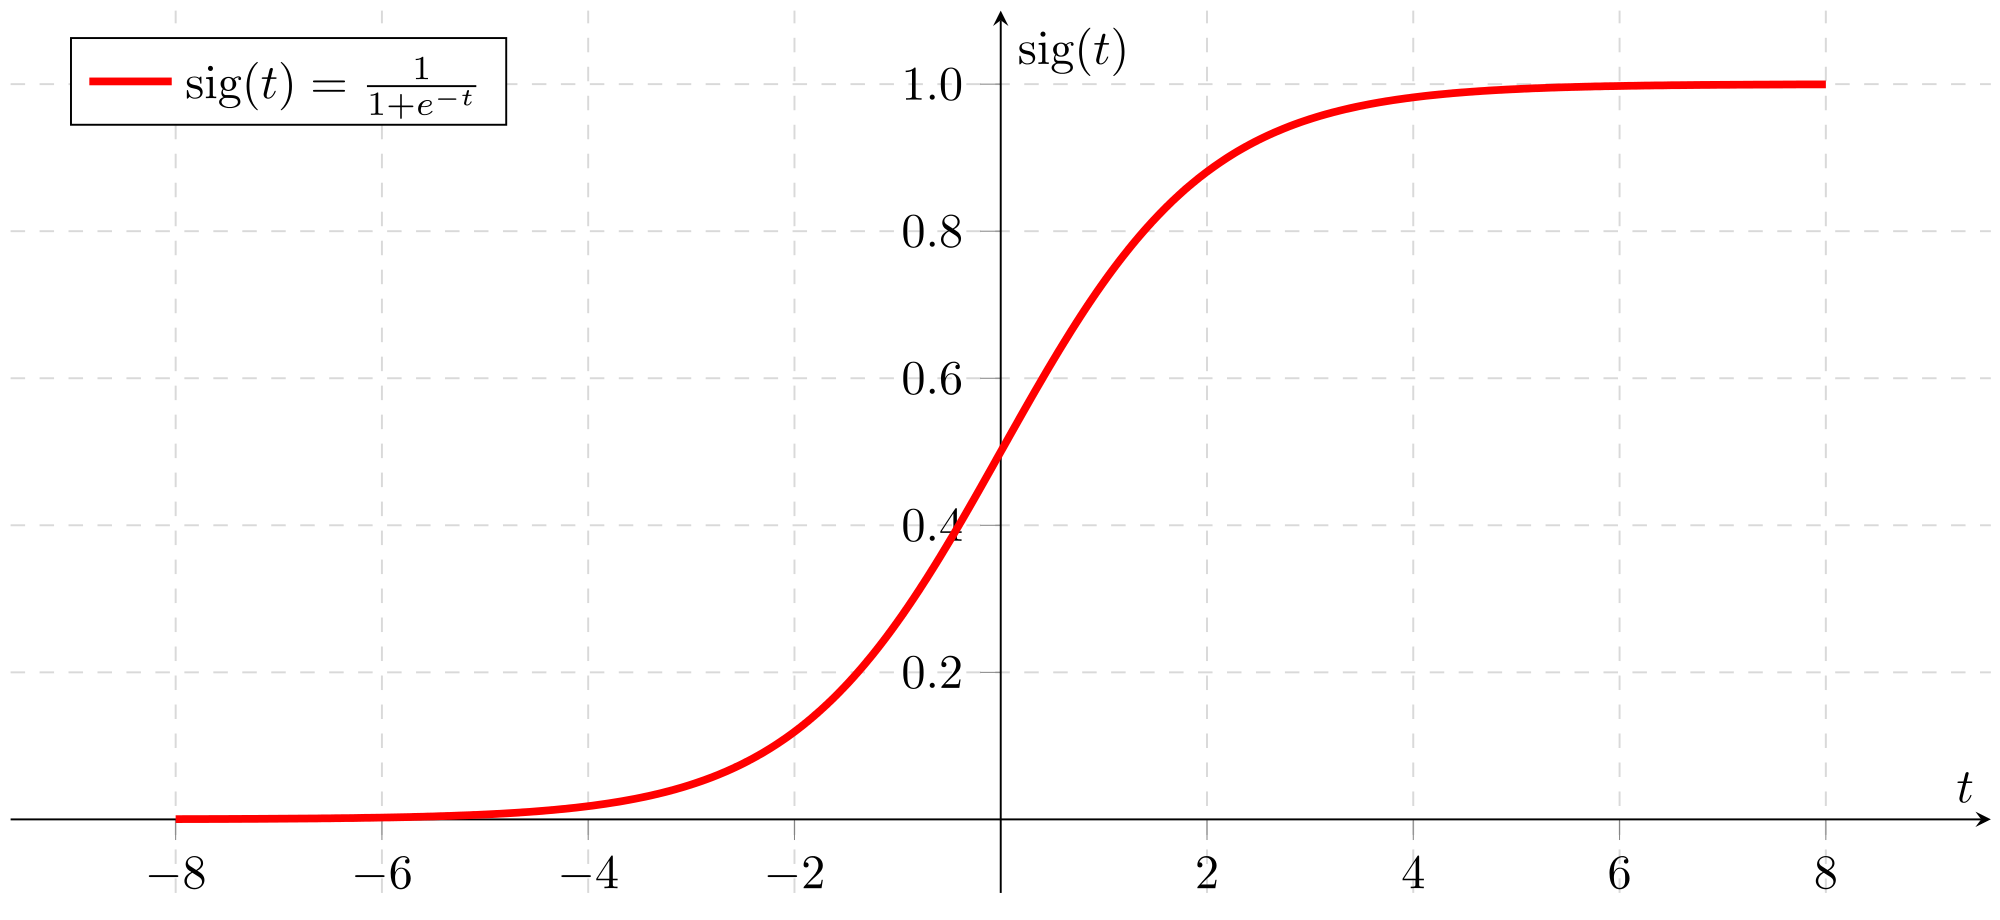
\includegraphics[width=25em]{figures/sigmoid}
    \caption{Sigmoid}
    \label{fig:sigmoid}
\end{figure}

$(\Vector{w}^T\Vector{x} + b)$ is a linear function $(a\Vector{x} + b)$, but since we are looking
for a probability constraint between [0, 1], the sigmoid function is used. The function is bounded
between [0, 1] as shown in the graph~\ref{fig:sigmoid}.

Some observations from the sigmoid function graph:
\begin{itemize}
    \item If $z$ is a large positive number, then $\sigma(z) = 1$
    \item If $z$ is small or large negative number, then $\sigma(z) = 0$
    \item If $z = 0$, then $\sigma(z) = 0.5$
\end{itemize}

\paragraph{Logistic Regression cost function}
$\hat{y}^{(i)} = \sigma (\Vector{w}^T \Vector{x}^{(i)} + b)$, where
$\sigma(z^{(i)}) = \frac{1}{1+e^{-z^{(i)}}}$

Given $\{(\Vector{x}^{(1)}, y^{(2)}), (\Vector{x}^{(2)}, y^{(2)}), \ldots,
(\Vector{x}^{(m)}, y^{(m)})\}$, want $\hat{y}^{(i)} \approx y^{(i)}$.

\paragraph{Loss (error) function:} (for single example)
\begin{IEEEeqnarray*}{rCl}
    \Cal{L}(\hat{y}, y) = -(y\log{\hat{y}} + (1-y)\log(1-\hat{y}))
\end{IEEEeqnarray*}

If $y = 1$: $\Cal{L}(\hat{y}, y) = -\log \hat{y}$ $\leftarrow$ want $\log \hat{y}$ large, want
$\hat{y}$ large.

If $y = 0$: $\Cal{L}(\hat{y}, y) = -\log(1-\hat{y})$ $\leftarrow$ want $\log(1-\hat{y})$ large,
want $\hat{y}$ small.

The loss function measures the discrepancy between the prediction ($\hat{y^{(i)}}$) and the desired
output ($y^{(i)}$). In other words, the loss function computes the error for a single training
example.

Note: Why can't use $\Cal{L}(\hat{y}, y) = \frac{1}{2}(\hat{y}-y)^2$? Because
$\Cal{L}(\hat{y}, y) = -(y\log{\hat{y}} + (1-y)\log(1-\hat{y}))$ is convex, however,
$\Cal{L}(\hat{y}, y) = \frac{1}{2}(\hat{y}-y)^2$ is non-convex.

\paragraph{Cost function:} (for entire training set)
\begin{IEEEeqnarray*}{rCl}
    J(\Vector{w}, b) = \frac{1}{m} \sum_{i=1}^m \Cal{L}(\hat{y}^{(i)}, y^{(i)}) = - \frac{1}{m}
    \sum_{i=1}^m[(y^{(i)}\log(\hat{y}^{(i)})) + (1-y^{(i)})\log(1-\hat{y}^{(i)})]
\end{IEEEeqnarray*}

The cost function is the average of the loss function of the entire training set. We are going to
find the parameters $\Vector{w}$ and $b$ that minimize the overall cost function.

\paragraph{Gradient Descent}
\begin{figure}[htb]
    \centering
    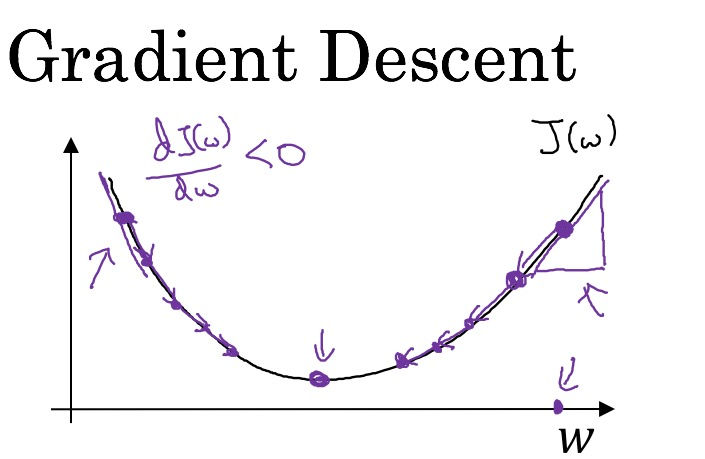
\includegraphics[width=25em]{figures/gradient-descent}
    \caption{Gradient descent. (Ignore $b$ here)}
\end{figure}

\begin{algorithm}[htb]
\Repeat{iteration = MaxIteration}{
        $\displaystyle{\Vector{w} := \Vector{w}
        - \alpha \frac{\partial J(\Vector{w}, b)}{\partial \Vector{w}}}$ \\
        $\displaystyle{b := b - \alpha \frac{\partial J(\Vector{w}, b)}{\partial b}}$
}
\end{algorithm}

Note: We often use ``d$\Vector{w}$'' to denote
$\displaystyle{\frac{\partial J(\Vector{w}, b)}{\partial \Vector{w}}}$, use
``d$b$'' to denote $\displaystyle{\frac{\partial J(\Vector{w}, b)}{\partial b}}$. In other words,
we use ``d$var$'' to denote $\displaystyle\frac{\text{d}FinalOutputVar}{\text{d}var}$ or
$\displaystyle\frac{\partial FinalOutputVar}{\partial var}$.

\paragraph{Gradient on single example:}
\begin{IEEEeqnarray*}{rCl}
    z = \Vector{w}^T \Vector{x} + b
\end{IEEEeqnarray*}

\begin{IEEEeqnarray*}{rCl}
    \hat{y} = a = \sigma(z) = \frac{1}{1 + e^{-z}}
\end{IEEEeqnarray*}

\begin{IEEEeqnarray*}{rCl}
    \Cal{L}(a, y) = -(y\log(a) + (1-y)\log(1-a))
\end{IEEEeqnarray*}

\begin{figure}[htb]
    \centering
    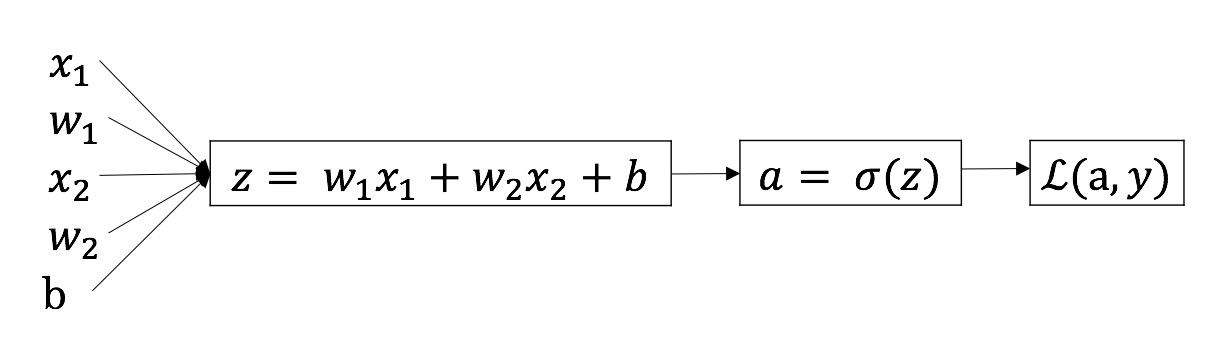
\includegraphics[width=35em]{figures/lr-gradient-descent}
    \caption{The computation graph of logistic regression gradient descent}
    \label{fig:lr-gradient-descent}
\end{figure}

According to the computation graph~\ref{fig:lr-gradient-descent}, go backwards to compute the
derivatives:
\begin{IEEEeqnarray*}{rCl}
    \text{d}a = \frac{\text{d}\Cal{L}(a, y)}{\text{d}a} = -\frac{y}{a} + \frac{1-y}{1-a}
\end{IEEEeqnarray*}

\begin{IEEEeqnarray*}{rCl}
    \text{d}z = \frac{\text{d}\Cal{L}(a, y)}{\text{d}z} = \frac{\text{d}\Cal{L}}{\text{d}a} \cdot
    \frac{\text{d}a}{\text{d}z} = (-\frac{y}{a} + \frac{1-y}{1-a}) \cdot a(1-a) = a - y
\end{IEEEeqnarray*}

\begin{IEEEeqnarray*}{rCl}
    \text{d}w_1 = \frac{\partial \Cal{L}}{\partial w_1} = x_1 \text{d}z = x_1 (a-y)
\end{IEEEeqnarray*}

\begin{IEEEeqnarray*}{rCl}
    \text{d}w_2 = \frac{\partial \Cal{L}}{\partial w_2} = x_2 \text{d}z = x_2 (a-y)
\end{IEEEeqnarray*}

\begin{IEEEeqnarray*}{rCl}
    \text{d}b = \frac{\partial \Cal{L}}{\partial b} = \text{d}z = a - y
\end{IEEEeqnarray*}

\paragraph{Gradient on m examples:}
\begin{IEEEeqnarray*}{rCl}
    J(\Vector{w}, b) = \frac{1}{m} \sum_{i=1}^m \Cal{L}(a^{(i)}, y^{(i)})
\end{IEEEeqnarray*}

\begin{IEEEeqnarray*}{rCl}
    a^{(i)} = \hat{y^{(i)}} = \sigma(z^{(i)}) = \sigma(\Vector{w}^T \Vector{x}^{(i)} + b)
\end{IEEEeqnarray*}

\begin{IEEEeqnarray*}{rCl}
    \frac{\partial J(\Vector{w}, b)}{\partial w_1} = \frac{1}{m} \sum_{i=1}^m
    \frac{\partial \Cal{L}(a^{(i)}, y^{(i)})}{\partial w_1} = \frac{1}{m} \sum_{i=1}^m
    \text{d}w_1^{(i)}
\end{IEEEeqnarray*}

The Algorithm~\ref{alg:lr_gradient_descent} is the algorithm of logistic regression gradient
descent on m examples. It uses two for-loops, so it's less efficient than use vertorization.

\begin{algorithm}[htb]
    \tcp{Initialization}
    $J = 0;$ \\
    \For{$j = 1$ \KwTo $n$}{
        $\text{d}w_j = 0$ \\
    }
    $\text{d}b = 0;$

    \tcp{Compute cost and derivatives}
    \For{$i = 0$ \KwTo $m$}{
        $z^{(i)} = \Vector{w}^T \Vector{x^{(i)}} + b;$ \\
        $a^{(i)} = \sigma(z^{(i)});$ \\
        $J = J - [y^{(i)} \log a^{(i)} + (1-y^{(i)})\log (1-a^{(i)})];$ \\
        $\text{d}z^{(i)} = a^{(i)} - y^{(i)};$ \\
        \For{$j = 1$ \KwTo $n$}{
            $\text{d}w_j = \text{d}w_j + x_j^{(i)} \text{d}z^{(i)};$ \\
        }
        $\text{d}b = \text{d}b + \text{d}z^{(i)}$
    }

    \tcp{Get the average}
    $J = J / m;$ \\
    \For{$j = 1$ \KwTo $n$}{
        $\text{d}w_j = \text{d}w_j / m$
    }
    $\text{d}b = \text{d}b / m;$

    \tcp{Gradient descent}
    \For{$j = 1$ \KwTo $n$}{
        $\text{d}w_j = \text{d}w_j - \alpha \text{d}w_j$
    }
    $b = b - \alpha \text{d}b$
    \caption{Logistic regression gradient descent on m examples}
    \label{alg:lr_gradient_descent}
\end{algorithm}

\pagebreak[6]

\subsection{Python and Vectorization}
\subsubsection{Vectorization}
\paragraph{What is vectorization?}
\begin{IEEEeqnarray*}{rCl}
    z = \Vector{w}^T \Vector{x} + b \qquad\qquad
    \Vector{w} = \left[\begin{array}{c}
        \vdots \\
        \vdots \\
    \end{array} \right], \qquad
    \Vector{x} = \left[\begin{array}{c}
        \vdots \\
        \vdots \\
    \end{array} \right], \qquad
    \Vector{w} \in \Set{R}^{n_x}, \quad
    \Vector{x} \in \Set{R}^{n_x}
\end{IEEEeqnarray*}

\begin{multicols}{2}
Non vectorized:
\begin{minted}{numpy}
    z = 0
    for i in range(n_x):
        z += w[i] * x[i]
    z += b
\end{minted}
\columnbreak

Vectorized:
\begin{minted}{numpy}
    z = np.dot(w, x) + b
\end{minted}
\end{multicols}

\begin{IEEEeqnarray*}{rCl}
    \left\{
        \begin{array}{r}
            \text{CPU} \\
            \text{GPU}
        \end{array}
    \right.
    \qquad \text{SIMD - Single Instruction Multiple Data}
\end{IEEEeqnarray*}

\subsubsection{More Vectorization Examples}
\paragraph{Neural network programming guideline}
Whenever possible, avoid explicit for-loops.

For example, compute $\Vector{u} = \Vector{A} \Vector{v}$. $\Vector{A} \in \Set{R}^{m \times n}$,
$\Vector{v} \in \Set{R}^{n}$.

\begin{multicols}{2}
Non-vectorized: $\displaystyle u_i = \sum_j \Vector{A}_{ij} v_j$
\begin{minted}{numpy}
    u = np.zeros((n, 1))
    for i in range(A.shape[0]):
        for j in range(A.shape[1]):
            u[i] += A[i][j] * v[j]
\end{minted}
\columnbreak
Vectorized:
\begin{minted}{numpy}
    u = np.dot(A, v)
\end{minted}
\end{multicols}

\paragraph{Vectors and matrix valued functions}
Say you need to apply the exponential operation on every element of a matrix/vector.
\begin{IEEEeqnarray*}{rCl}
    \Vector{v} = \left[
        \begin{array}{c}
            v_1 \\
            \vdots \\
            v_n
        \end{array}
    \right]
    \longrightarrow
    \Vector{u} = \left[
        \begin{array}{c}
            e^{v_1} \\
            \vdots \\
            e^{v_n}
        \end{array}
    \right]
\end{IEEEeqnarray*}

\begin{multicols}{2}
Non-vectorized:
\begin{minted}{numpy}
    u = np.zeors((n, 1))
    for i in range(n):
        u[i] = math.exp(v[i])
\end{minted}
\columnbreak
Vectorized:
\begin{minted}{numpy}
    u = np.exp(v)
\end{minted}
\end{multicols}

\paragraph{Logistic regression derivatives}
\begin{algorithm}[htb]
    J = 0 \\
    \tcp{$\text{d}w_1 = 0, \text{d}w_2 = 0, \ldots, \text{d}w_{n_x}$}
    $\text{d}\Vector{w}$ = np.zeros(($n_x$, 1)) \\
    $\text{d}b$ = 0 \\
    \For{$i = 1$ \KwTo $m$}{
        $z^{(i)} = \Vector{w}^T x^{(i)} + b$ \\
        $a^{(i)} = \sigma(z^{(i)})$ \\
        $J = J - [y^{(i)}\log \hat{y}^{(i)} + (1-y^{(i)})\log (1-\hat{y}^{(i)})]$ \\
        $\text{d}z^{(i)} = a^{(i)} - y^{(i)}$ \\
        \tcp{
            $\text{d}w_1 = \text{d}w_1 + x_1^{(i)} \text{d}z^{(i)}$ \\
            $\text{d}w_2 = \text{d}w_2 + x_2^{(i)} \text{d}z^{(i)}$ \\
            \ldots \\
            $\text{d}w_{n_x} = \text{d}w_{n_x} + x_{n_x}^{(i)} \text{d}z^{(i)}$
        }
        $\text{d}\Vector{w} = \text{d}\Vector{w} + x^{(i)}\text{d}z^{(i)}$ \\
        $\text{d}b = \text{d}b + \text{d}z^{(i)}$ \\
    }
    $J = J / m$ \\
    \tcp{
        $\text{d}w_1 = \text{d}w_1 / m$ \\
        $\text{d}w_2 = \text{d}w_2 / m$ \\
        \ldots \\
        $\text{d}w_{n_x} = \text{d}w_{n_x} / m$
    }
    $\text{d}\Vector{w} = \text{d}\Vector{w} / m$ \\
    $\text{d}b = \text{d}b / m$
    \caption{Replace the inner for-loop by vectorization in logistic regression}
\end{algorithm}

\subsubsection{Vectorizing Logistic Regression}
Inference process:
\begin{IEEEeqnarray*}{rCl}
    z^{(1)} = \Vector{w}^T \Vector{x^{(1)}} + b \qquad z^{(2)} = \Vector{w}^T \Vector{x^{(2)}} + b
    \qquad \cdots \qquad z^{(m)} = \Vector{w}^T \Vector{x^{(m)}} + b
\end{IEEEeqnarray*}
\begin{IEEEeqnarray*}{rCl}
    a^{(1)} = \sigma (z^{(1)}) \qquad a^{(2)} = \sigma (z^{(2)}) \qquad \cdots \qquad
    a^{(m)} = \sigma (z^{(m)})
\end{IEEEeqnarray*}
\begin{IEEEeqnarray*}{rCl}
    \Matrix{X} = \left[
        \begin{array}{cccc}
            \vRule & \vRule & & \vRule \\
            \Vector{x^{(1)}} & \Vector{x^{(2)}} & \cdots & \Vector{x^{(m)}} \\
            \vRule & \vRule & & \vRule
        \end{array}
    \right]
    \qquad
    \Matrix{X} \in \Set{R}^{{n_x} \times m}
\end{IEEEeqnarray*}
\begin{IEEEeqnarray*}{rCl}
    \Vector{Z} = \left[
        \begin{array}{cccc}
            z^{(1)} & z^{(2)} & \cdots & z^{(m)}
        \end{array}
    \right]
    = \Vector{w}^T \Matrix{X}
    + \underbrace{\left[\begin{array}{cccc}
        b & b & \cdots & b
    \end{array}\right]}_{1 \times m}
\end{IEEEeqnarray*}
\begin{IEEEeqnarray*}{rCl}
    \Vector{A} = \left[
        \begin{array}{cccc}
            a^{(1)} & a^{(2)} & \cdots & a^{(m)}
        \end{array}
    \right]
    = \sigma(\Vector{Z})
\end{IEEEeqnarray*}

\begin{IEEEeqnarray*}{rCl}
    \text{d}z^{(1)} = a^{(1)} - y^{(1)} \qquad \text{d}z^{(2)} = a^{(2)} - y^{(2)} \qquad \cdots
    \qquad \text{d}z^{(m)} = a^{(m)} - y^{(m)}
\end{IEEEeqnarray*}

\begin{IEEEeqnarray*}{rCl}
    \text{d}\Vector{Z} = \left[
        \begin{array}{cccc}
            \text{d}z^{(1)} & \text{d}z^{(2)} & \cdots & \text{d}z^{(m)}
        \end{array}
    \right]
\end{IEEEeqnarray*}

\begin{IEEEeqnarray*}{rCl}
    \Vector{Y} = \left[
        \begin{array}{cccc}
            y^{(1)} & y^{(2)} & \cdots & y^{(m)}
        \end{array}
    \right]
\end{IEEEeqnarray*}

\begin{IEEEeqnarray*}{rCl}
    \text{d}\Vector{Z} = \Vector{A} - \Vector{Y} = \left[
        \begin{array}{cccc}
            a^{(1)}-y^{(1)} & a^{(2)}-y^{(2)} & \cdots & a^{(m)}-y^{(m)}
        \end{array}
    \right]
\end{IEEEeqnarray*}

\begin{IEEEeqnarray*}{rCl}
    \text{d}b = \frac{1}{m} \sum_{i=1}^m \text{d}z^{(i)}
    \longrightarrow
    \text{d}b = \frac{1}{m} \text{np.sum(}\text{d}\Vector{Z}\text{)}
\end{IEEEeqnarray*}

\begin{IEEEeqnarray*}{rCl}
    \text{d}\Vector{w} = \frac{1}{m} \left[
        \begin{array}{cccc}
            \vRule & \vRule & & \vRule \\
            \Vector{x^{(1)}} & \Vector{x^{(2)}} & \cdots & \Vector{x^{(m)}} \\
            \vRule & \vRule & & \vRule
        \end{array}
    \right]
    \left[
        \begin{array}{c}
            \text{d}z^{(1)} \\
            \text{d}z^{(2)} \\
            \vdots \\
            \text{d}z^{(m)}
        \end{array}
    \right]
    = \frac{1}{m} \underbrace{\left[
        \Vector{x}^{(1)}\text{d}z^{(1)} + \Vector{x}^{(2)}\text{d}z^{(2)} + \cdots
        + \Vector{x}^{(m)}\text{d}z^{(m)}
    \right]}_{n \times 1}
    \longrightarrow
    \text{d}\Vector{w} = \frac{1}{m} \Matrix{X} \text{d}\Vector{Z}^T
\end{IEEEeqnarray*}

Vectorized (in a single iteration):
\begin{IEEEeqnarray*}{rCl}
    \Vector{Z} = \Vector{w}^T\Matrix{X} + b \longrightarrow \text{np.dot(w.T, X) + b}
\end{IEEEeqnarray*}
\begin{IEEEeqnarray*}{rCl}
    \Vector{A} = \sigma(\Vector{Z})
\end{IEEEeqnarray*}
\begin{IEEEeqnarray*}{rCl}
    \text{d}\Vector{Z} = \Vector{A} - \Vector{Y}
\end{IEEEeqnarray*}
\begin{IEEEeqnarray*}{rCl}
    \text{d}\Vector{w} = \frac{1}{m} \Matrix{X}(\text{d}\Vector{Z}^T)
\end{IEEEeqnarray*}
\begin{IEEEeqnarray*}{rCl}
    \text{d}b = \frac{1}{m} \text{np.sum(d}\Vector{Z}\text{)}
\end{IEEEeqnarray*}

Then update $\Vector{w}$ and $b$ for each iteration:
\begin{IEEEeqnarray*}{rCl}
    \Vector{w} = \Vector{w} - \alpha \text{d}\Vector{w}
\end{IEEEeqnarray*}
\begin{IEEEeqnarray*}{rCl}
    b = b - \alpha \text{d}b
\end{IEEEeqnarray*}

\subsubsection{Broadcasting in Python}
According to Figure~\ref{fig:foods-calories}, denote the matrix in the figure as $\Matrix{A}$,
calculate the percentages of calories from Carbs, Proteins, Fats for each of four foods. Try do that
without explicit for-loop.

\begin{figure}[htb]
    \centering
    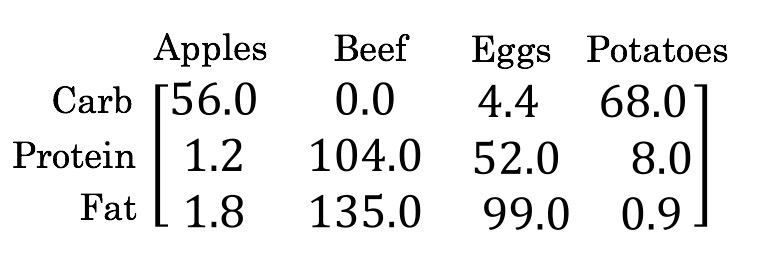
\includegraphics[width=25em]{figures/foods-calories}
    \caption{Calories from Carbs, Proteins, Fats in 100g of different foods}
    \label{fig:foods-calories}
\end{figure}

\begin{minted}{numpy}
    cal = A.sum(axis=0) # sum vertically, pass axis=1 to sum horizontally
    # broadcasting, A.shape = (3, 4), cal.shape = (1, 4)
    percentage = 100 * A / (cal.reshape(1, 4))
\end{minted}

\paragraph{Broadcasting examples}
\begin{IEEEeqnarray*}{rCl}
    \left[\begin{array}{c} 1 \\ 2 \\ 3 \\ 4 \end{array}\right] + 100
    = \left[\begin{array}{c} 1 \\ 2 \\ 3 \\ 4 \end{array}\right]
    + \left[\begin{array}{c} 100 \\ 100 \\ 100 \\ 100 \end{array} \right]
    = \left[\begin{array}{c} 101 \\ 102 \\ 103 \\ 104 \end{array} \right]
\end{IEEEeqnarray*}

\begin{IEEEeqnarray*}{rCl}
    \left[\begin{array}{ccc} 1 & 2 & 3 \\ 4 & 5 & 6 \end{array}\right]
    + \left[\begin{array}{ccc} 100 & 200 & 300 \end{array}\right]
    = \left[\begin{array}{ccc} 1 & 2 & 3 \\ 4 & 5 & 6 \end{array}\right]
    + \left[\begin{array}{ccc} 100 & 200 & 300 \\ 100 & 200 & 300 \end{array}\right]
    = \left[\begin{array}{ccc} 101 & 202 & 303 \\ 104 & 205 & 306 \end{array}\right]
\end{IEEEeqnarray*}

\begin{IEEEeqnarray*}{rCl}
    \left[\begin{array}{ccc} 1 & 2 & 3 \\ 4 & 5 & 6 \end{array}\right]
    + \left[\begin{array}{c} 100 \\ 200 \end{array}\right]
    = \left[\begin{array}{ccc} 1 & 2 & 3 \\ 4 & 5 & 6 \end{array}\right]
    + \left[\begin{array}{ccc} 100 & 100 & 100 \\ 200 & 200 & 200 \end{array}\right]
\end{IEEEeqnarray*}

(Note: In MATLAB/Octave, the \mintinline{matlab}{bsxfun} seems to have the same feature, it can
apply element-wise operation to two arrays with implicit expansion enabled.)

\paragraph{General principle of broadcasting}
\begin{IEEEeqnarray*}{rCl}
    \underbrace{\Matrix{Matrix}}_{(m, n)} \qquad
    \begin{array}{c} + \\ - \\ * \\ / \end{array} \qquad
    \underbrace{\Vector{Vector}}_{(1, n) or (m, 1)} \qquad
    \longrightarrow  \qquad \underbrace{\Matrix{Matrix}}_{(m, n)}
\end{IEEEeqnarray*}

\subsubsection{A Note on Python/NumPy Vectors}
For broadcasting:
\begin{IEEEeqnarray*}{rCl}
    \left\{\begin{array}{rl}
        \text{Strenght:} & \text{expressivity, flexibility} \\
        \text{Weakness:} & \text{may introduce subtle bugs}
    \end{array}\right.
\end{IEEEeqnarray*}

\begin{minted}{numpy}
    >>> import numpy as np
    >>> a = np.random.randn(5)
    >>> a   # rank 1 array, do not use in this course
    array([-0.40700705, -1.27728182,  0.10255894,  0.06871343, -1.01614418])
    >>> a.shape
    (5,)
    >>> a = a.reshape((5, 1))       # column vector
    >>> a
    array([[-0.40700705],
           [-1.27728182],
           [ 0.10255894],
           [ 0.06871343],
           [-1.01614418]])
    >>> a = np.random.randn(5, 1)   # column vector
    >>> a
    array([[ 1.32238445],
           [-2.09932992],
           [ 0.29040232],
           [-1.31295795],
           [-1.05893313]])
    >>> a.shape
    (5, 1)
    >>> a = np.random.randn(1, 5)   # row vector
    >>> a
    array([[-0.7020727 , -0.54867968,  1.38088584,  0.69785511, -0.2510519 ]])
    >>> a.shape
    (1, 5)
    >>> assert(a.shape == (1, 5))
    >>> assert(a.shape == (5, 1))
    Traceback (most recent call last):
      File "<stdin>", line 1, in <module>
    AssertionError
\end{minted}

\subsubsection{Explanation of Logistic Regression Cost Function (Optional)}
Logistic regression cost function:
\begin{IEEEeqnarray*}{rCl}
    \hat{y} = \sigma(\Vector{w}^T \Vector{x} + b), \qquad
    \text{where } \sigma(z) = \frac{1}{1+e^{-z}}.
\end{IEEEeqnarray*}

\begin{IEEEeqnarray*}{rCl}
    \left.\begin{array}{rl}
        \text{If }y=1\text{: } & P(y|x) = \hat{y} \\
        \text{If }y=0\text{: } & P(y|x) = 1 - \hat{y}
    \end{array}\right\}
    P(y|x) = \hat{y}^y (1-\hat{y})^{(1-y)}
\end{IEEEeqnarray*}

\begin{IEEEeqnarray*}{rCl}
    \log P(y|x) = y \log\hat{y} + (1-y)\log(1-\hat{y}) = -\Cal{L}(\hat{y}, y)
\end{IEEEeqnarray*}

Cost on m examples: (Maximum Likelihood Estimation)
\begin{IEEEeqnarray*}{rCl}
    \log P(\text{labels in training set}) = \log \prod_{i=1}^m P(y^{(i)}|x^{(i)})
    = \underbrace{\sum_{i=1}^m \log P(y^{(i)}|x^{(i)})}_{-\Cal{L}(\hat{y}^{(i)}, y^{(i)})}
    = -\sum_{(i=1)}^m \Cal{L}(\hat{y}^{(i)}, y^{(i)})
\end{IEEEeqnarray*}

\begin{IEEEeqnarray*}{rCl}
    \underset{\text{minimize}}{J(\Vector{w}, b)}
    = \frac{1}{m} \sum_{i=1}^m \Cal{L}(\hat{y}^{(i)}, y^{(i)})
\end{IEEEeqnarray*}

\section{Shallow Neural Network}
\subsection{Neural Network Overview}
\begin{figure}[htb]
    \centering
    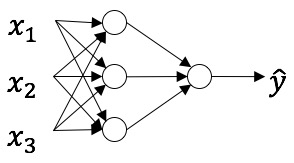
\includegraphics[width=15em]{figures/shallow-nn}
    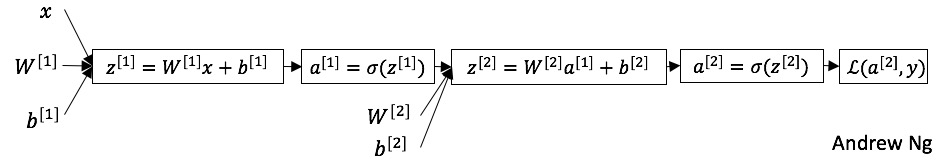
\includegraphics[width=50em]{figures/shallow-nn-compute}
    \caption{The example of a shallow neural network}
    \label{fig:shallow-nn}
\end{figure}

Figure~\ref{fig:shallow-nn} shows an example of a shallow neural network.

Notation: Use superscript $[i]$ to denote the i-th layer; use the superscript $(i)$ to denote the
i-th example in dataset.

\subsection{Neural Network Representation}
As is shown in Figure~\ref{fig:nn-representation}, $\Vector{a^{[i]}}$ denotes the activation of the
i-th layer.
\begin{figure}[htb]
    \centering
    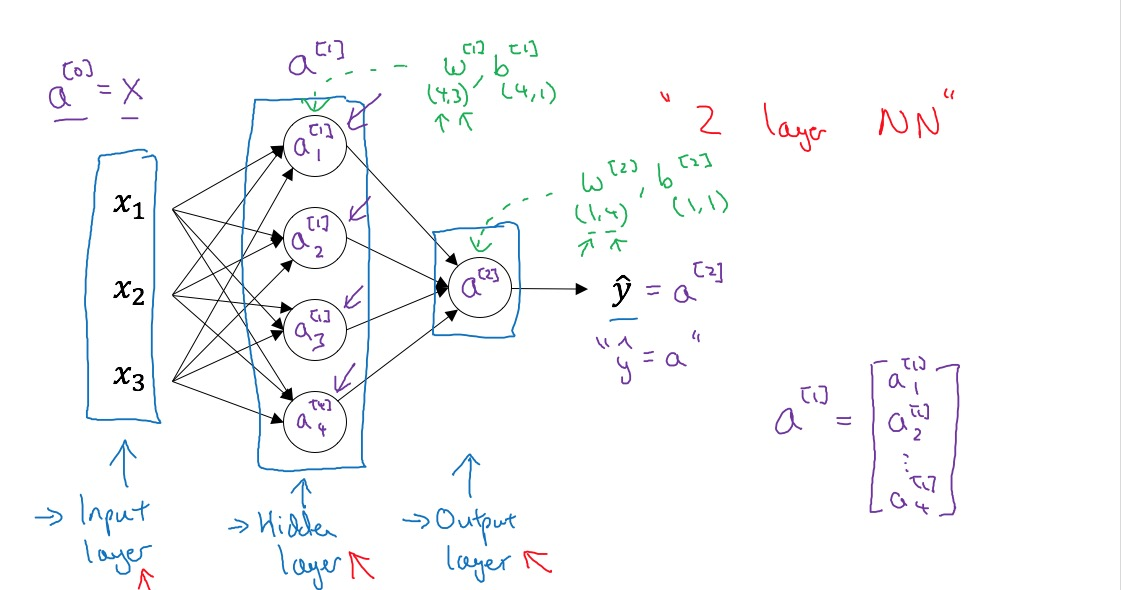
\includegraphics[width=40em]{figures/nn-representation}
    \caption{The representation of a neural network}
    \label{fig:nn-representation}
\end{figure}

\subsection{Computing a Neural Network's Output}
As the Figure~\ref{fig:neuron-compuation} shows, the compuation of a single neuron includes two
parts: the first part, $\Vector{z} = \Vector{w}^T\Vector{x} + b$; the second part,
$\Vector{a} = \sigma(\Vector{z})$.
\begin{figure}[htb]
    \centering
    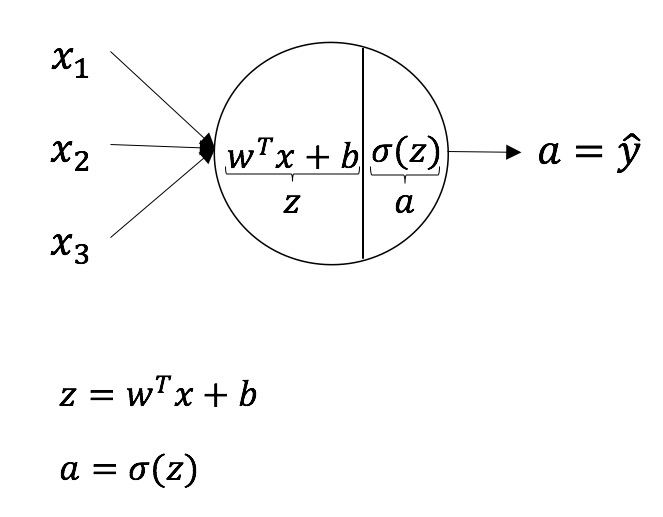
\includegraphics[width=20em]{figures/neuron-computation}
    \caption{The computation of a single neuron}
    \label{fig:neuron-compuation}
\end{figure}

\begin{figure}[htb]
    \centering
    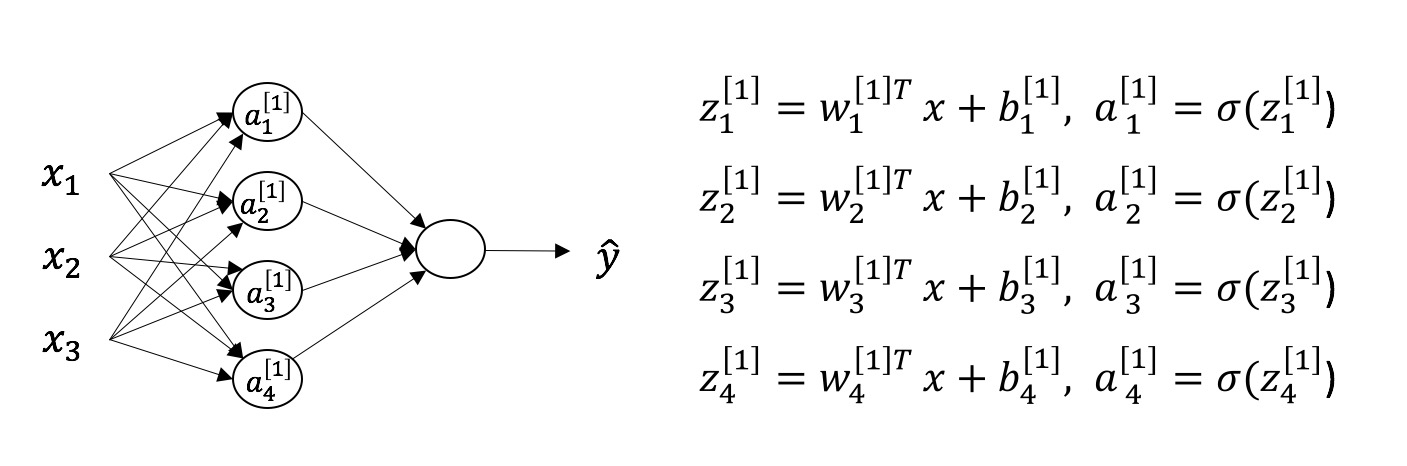
\includegraphics[width=40em]{figures/nn-first-layer-computation}
    \caption{The computation of the first layer of a neural network}
    \label{fig:nn-first-layer-computation}
\end{figure}

The Figure~\ref{fig:nn-first-layer-computation} shows the compuation of the neural network's first
layer. Cause it uses a for-loop, it is less efficient. According to it, we can generize a
vectorized version:
\begin{IEEEeqnarray*}{rCl}
    \Vector{z^{[1]}} = \left[\begin{array}{c}
        z_1^{[1]} \\ z_2^{[1]} \\ z_3^{[1]} \\ z_4^{[1]}
    \end{array}\right] \qquad
    \Matrix{W^{[1]}} = \left[\begin{array}{c}
        \hRule \Vector{w_1^{[1]}}^T \hRule \\
        \hRule \Vector{w_2^{[1]}}^T \hRule \\
        \hRule \Vector{w_3^{[1]}}^T \hRule \\
        \hRule \Vector{w_4^{[1]}}^T \hRule
    \end{array}\right] \qquad
    \Vector{x} = \Vector{a^{[0]}} = \left[\begin{array}{c}
        x_1 \\ x_2 \\ x_3
    \end{array}\right] \qquad
    \Vector{b} = \left[\begin{array}{c}
        b_1^{[1]} \\ b_2^{[1]} \\ b_3^{[1]} \\ b_4^{[1]}
    \end{array}\right]
\end{IEEEeqnarray*}

Given input $\Vector{x} (\Vector{a^{[0]}})$:
\begin{IEEEeqnarray*}{rCl}
    \Vector{z^{[1]}} = \Matrix{W^{[1]}} \Vector{a^{[0]}} + \Vector{b^{[1]}} \qquad
    \Vector{a^{[1]}} = \sigma(\Vector{z^{[1]}}) \qquad
    \Vector{z^{[2]}} = \Matrix{W^{[2]}} \Vector{a^{[1]}} + \Vector{b^{[2]}} \qquad
    \Vector{a^{[2]}} = \sigma(\Vector{z^{[2]}})
\end{IEEEeqnarray*}

\subsection{Vectorizing across Multiple Examples}
For single example:
\begin{IEEEeqnarray*}{rCl}
    \Vector{x} \longrightarrow \Vector{a^{[2]}} = \Vector{\hat{y}}
\end{IEEEeqnarray*}

For m examples:
\begin{IEEEeqnarray*}{rCl}
    \Vector{x^{(1)}} \longrightarrow \Vector{a^{[2](1)}} = \Vector{\hat{y}^{(1)}} \qquad
    \Vector{x^{(2)}} \longrightarrow \Vector{a^{[2](2)}} = \Vector{\hat{y}^{(2)}} \qquad
    \ldots \qquad
    \Vector{x^{(m)}} \longrightarrow \Vector{a^{[2](m)}} = \Vector{\hat{y}^{(m)}} \qquad
\end{IEEEeqnarray*}

Non-vectorized:
\begin{algorithm}[htb]
    \For{$i = 1$ \KwTo $m$}{
        $\Vector{z^{[1](i)}} = \Matrix{W^{[1]}}\Vector{x^{(i)}} + \Vector{b^{[1]}}$ \\
        $\Vector{a^{[1](i)}} = \sigma(\Vector{z^{[1](1)}})$ \\
        $\Vector{z^{[2](1)}} = \Matrix{W^{[2]}}\Vector{a^{[1](i)}} + \Vector{b^{[2]}}$ \\
        $\Vector{a^{[2](i)}} = \sigma(\Vector{z^{[2](i)}})$
    }
\end{algorithm}

\begin{IEEEeqnarray*}{rCl}
    \text{Let} \quad \Matrix{X} = \underbrace{\left[\begin{array}{cccc}
        \vRule & \vRule & & \vRule \\
        \Vector{x^{(1)}} & \Vector{x^{(2)}} & \cdots & \Vector{x^{(m)}} \\
        \vRule & \vRule & & \vRule
    \end{array}\right]}_{(n_x, m)}
\end{IEEEeqnarray*}

\begin{IEEEeqnarray*}{rCl}
    \text{then} \quad \Matrix{Z^{[1]}} = \underbrace{\left[\begin{array}{cccc}
        \vRule & \vRule & & \vRule \\
        \Vector{z^{[1](1)}} & \Vector{z^{[1](2)}} & \cdots & \Vector{z^{[1](m)}} \\
        \vRule & \vRule & & \vRule
    \end{array}\right]}_{(\text{hidden units}, \text{training examples})} \qquad
    \Matrix{A^{[1]}} = \underbrace{\left[\begin{array}{cccc}
        \vRule & \vRule & & \vRule \\
        \Vector{a^{[1](1)}} & \Vector{a^{[1](2)}} & \cdots & \Vector{a^{[1](m)}} \\
        \vRule & \vRule & & \vRule
    \end{array}\right]}_{(\text{hidden units}, \text{training examples})}
\end{IEEEeqnarray*}

Vectorized:
\begin{IEEEeqnarray*}{rCl}
    \Matrix{Z^{[1]}} = \Matrix{W^{[1]}} \Matrix{A^{[0]}} + \Vector{b^{[1]}}
    = \Matrix{W^{[1]}} \Matrix{X} + \Vector{b^{[1]}}
\end{IEEEeqnarray*}
\begin{IEEEeqnarray*}{rCl}
    \Matrix{A^{[1]}} = \sigma(\Matrix{Z^{[1]}})
\end{IEEEeqnarray*}
\begin{IEEEeqnarray*}{rCl}
    \Matrix{Z^{[2]}} = \Matrix{W^{[2]}} \Matrix{A^{[1]}} + \Vector{b^{[2]}}
\end{IEEEeqnarray*}
\begin{IEEEeqnarray*}{rCl}
    \Matrix{A^{[2]}} = \sigma(\Matrix{Z^{[2]}})
\end{IEEEeqnarray*}

\subsection{Explanation for Vectorized Implementation}
\begin{IEEEeqnarray*}{rCl}
    \Vector{z^{[1](1)}} = \Matrix{W^{[1]}}\Vector{x^{(1)}} + \Vector{b^{[1]}}, \quad
    \Vector{z^{[1](2)}} = \Matrix{W^{[1]}}\Vector{x^{(2)}} + \Vector{b^{[1]}}, \quad
    \ldots, \quad
    \Vector{z^{[1](m)}} = \Matrix{W^{[1]}}\Vector{x^{(m)}} + \Vector{b^{[1]}}
\end{IEEEeqnarray*}

\begin{IEEEeqnarray*}{rCl}
    \Matrix{W^{[1]}} = \left[\begin{array}{c}
        \hRule \Vector{w_1^{[1]}}^T \hRule \\
        \hRule \Vector{w_2^{[1]}}^T \hRule \\
        \hRule \Vector{w_3^{[1]}}^T \hRule \\
        \hRule \Vector{w_4^{[1]}}^T \hRule
    \end{array}\right]
\end{IEEEeqnarray*}
\begin{IEEEeqnarray*}{rCl}
    \Matrix{W^{[1]}}{\color{purple} \Vector{x^{(1)}}} = {\color{purple} \left[\begin{array}{c}
        \cdot \\ \cdot \\ \cdot \\ \cdot
    \end{array}\right]} \qquad
    \Matrix{W^{[1]}}{\color{green} \Vector{x^{(2)}}} = {\color{green} \left[\begin{array}{c}
        \cdot \\ \cdot \\ \cdot \\ \cdot
    \end{array}\right]} \qquad
    \cdots \qquad
    \Matrix{W^{[1]}}{\color{yellow} \Vector{x^{(m)}}} = {\color{yellow} \left[\begin{array}{c}
        \cdot \\ \cdot \\ \cdot \\ \cdot
    \end{array}\right]}
\end{IEEEeqnarray*}
\begin{IEEEeqnarray*}{rCl}
    \Matrix{W^{[1]}}
    \left[
    {\color{purple}\begin{array}{c} \vRule \\ \Vector{x^{(1)}} \\ \vRule \end{array}}
    {\color{green}\begin{array}{c} \vRule \\ \Vector{x^{(2)}} \\ \vRule \end{array}}
    \cdots
    {\color{yellow}\begin{array}{c} \vRule \\ \Vector{x^{(m)}} \\ \vRule \end{array}}
    \right] + \Vector{b^{[1]}}
    = \left[{\color{purple} \begin{array}{c} \cdot \\ \cdot \\ \cdot \\ \cdot \end{array}}
    {\color{green} \begin{array}{c} \cdot \\ \cdot \\ \cdot \\ \cdot \end{array}} \cdots
    {\color{yellow} \begin{array}{c} \cdot \\ \cdot \\ \cdot \\ \cdot \end{array}}\right]
    + \Vector{b^{[1]}}
    = \left[
    {\color{purple}\begin{array}{c} \vRule \\ \Vector{z^{[1](1)}} \\ \vRule \end{array}}
    {\color{green}\begin{array}{c} \vRule \\ \Vector{z^{[1](2)}} \\ \vRule \end{array}}
    \cdots
    {\color{yellow}\begin{array}{c} \vRule \\ \Vector{z^{[1](m)}} \\ \vRule \end{array}}
    \right] = \Matrix{Z^{[1]}}
\end{IEEEeqnarray*}

So, $\Matrix{W^{[1]}\Vector{x^{(i)}}} + \Vector{b^{[1]}} = \Vector{z^{[1](i)}}$,
$\Matrix{Z^{[1]}} = \Matrix{W^{[1]}}\Matrix{X} + \Vector{b^{[1]}}$.

\subsection{Activation Functions}
Given $\Vector{x}$:
\begin{IEEEeqnarray*}{rCl}
    \Vector{z^{[1]}} = \Matrix{W^{[1]}}\Vector{x} + \Vector{b^{[1]}}
\end{IEEEeqnarray*}
{\centering \sout{$\Vector{a^{[1]}} = \sigma(\Vector{z^{[1]}})$} \par}
\begin{IEEEeqnarray*}{rCl}
    \Vector{a^{[1]}} = g^{[1]}(\Vector{z^{[1]}})
\end{IEEEeqnarray*}
\begin{IEEEeqnarray*}{rCl}
    \Vector{z^{[2]}} = \Matrix{W^{[2]}}\Vector{a^{[1]}} + b^{[2]}
\end{IEEEeqnarray*}
{\centering \sout{$\Vector{a^{[2]}} = \sigma(\Vector{z^{[2]}})$} \par}
\begin{IEEEeqnarray*}{rCl}
    \Vector{a^{[2]}} = g^{[2]}(\Vector{z^{[2]}})
\end{IEEEeqnarray*}

We use $g(z)$ to denote activation function. Sometimes we can use other activation function like
$tanh(z)$, ReLU ($max(0, z)$), etc., instead of $\sigma(z)$ function. Different layers of the
neural network may have different activation function, so we can use $g^{[i]}(z)$ to denote the
i-th layer's activation function of a neural network.

\subsubsection{Pros and cons of activation functions}
\begin{figure}[htb]
    \centering
    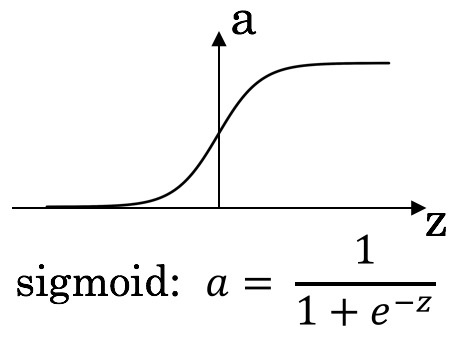
\includegraphics[width=20em]{figures/sigmoid-black} \qquad
    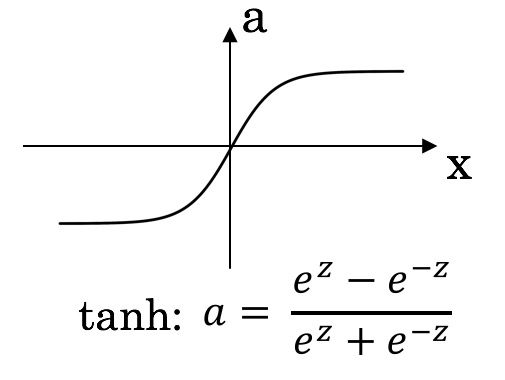
\includegraphics[width=19em]{figures/tanh} \\
    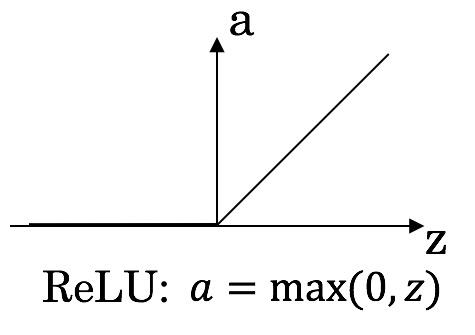
\includegraphics[width=20em]{figures/relu} \quad
    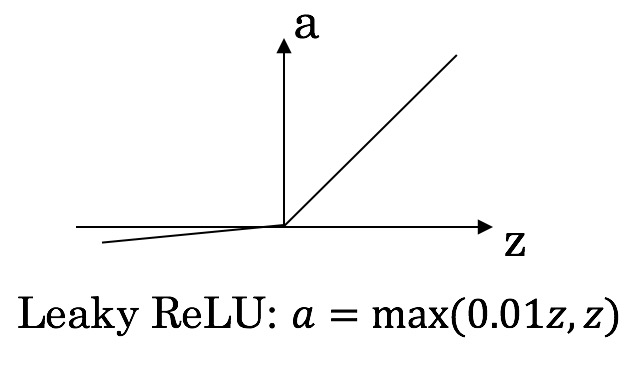
\includegraphics[width=24em]{figures/leaky-relu}
    \caption{Activation functions}
\end{figure}

\begin{itemize}
    \item One of downside of both the sigmoid and tanh activation function is that if $z$ is either
    very large or very small, then the gradient (derivative, slope) of the function becomes very
    small, this slows down the gradient descent.
    \item Never use sigmoid activation function, except for the output layer if you are doing
    binary classification. Tanh is prety superior than sigmoid.
    \item If you don't have an idea to choose which activation function, choose ReLU as the default
    activation function, or you can try Leaky ReLU.
\end{itemize}

\subsection{Why do you need non-linear activation functions?}
If $g(z) = z$, sometimes we will call it ``linear activation function'' or ``identity activation
function''.

Given $\Vector{x}$:
\begin{IEEEeqnarray*}{rCl}
    \Vector{z^{[1]}} = \Matrix{W^{[1]}}\Vector{x} + \Vector{b^{[1]}}
\end{IEEEeqnarray*}
\begin{IEEEeqnarray*}{rCl}
    \Vector{a^{[1]}} = g^{[1]}(\Vector{z^{[1]}}) = \Vector{z^{[1]}}
    = \Matrix{W^{[1]}}\Vector{x} + \Vector{b^{[1]}}
\end{IEEEeqnarray*}
\begin{IEEEeqnarray*}{rCl}
    \Vector{z^{[2]}} = \Matrix{W^{[2]}}\Vector{a^{[1]}} + b^{[2]}
    = \Matrix{W^{[2]}}(\Matrix{W^{[1]}}\Vector{x} + \Vector{b^{[1]}}) + \Vector{b^{[2]}}
    = \underbrace{(\Matrix{W^{[2]}}\Matrix{W^{[1]}})}_{\Matrix{W'}}\Vector{x}
    + \underbrace{(\Matrix{W^{[2]}}\Vector{b^{[1]}} + \Vector{b^{[2]}})}_{\Vector{b'}}
    = \Matrix{W'}\Vector{x} + \Vector{b'}
\end{IEEEeqnarray*}
\begin{IEEEeqnarray*}{rCl}
    \Vector{a^{[2]}} = g^{[2]}(\Vector{z^{[2]}}) = \Vector{z^{[2]}}
    = \Matrix{W'}\Vector{x} + \Vector{b'}
\end{IEEEeqnarray*}

If you use linear activation function as the activation function of your neural network, then the
neural network is just outputting a linear function of the input. It turns out that if you use a
linear function or alternatively if you don't have an activation function, then no matter how many
layers your neural network has always doing is just computing a linear activation function, so you
might as well not have any hidden layers.

\subsection{Derivatives of activation functions}
\subsubsection{Sigmoid activation function}
\begin{IEEEeqnarray*}{rCl}
    g(z) = \frac{1}{1+e^{-z}} = a
\end{IEEEeqnarray*}
\begin{IEEEeqnarray*}{rCl}
    g'(z) = \frac{\text{d}}{\text{d}z}g(z) = \frac{1}{1+e^{-z}}(1-\frac{1}{1+e^{-z}})
    = g(z)(1-g(z)) = a(1-a)
\end{IEEEeqnarray*}
\subsubsection{Tanh activation function}
\begin{IEEEeqnarray*}{rCl}
    g(z) = \tanh(z) = \frac{e^z-e^{-z}}{e^z+e^{-z}} = a
\end{IEEEeqnarray*}
\begin{IEEEeqnarray*}{rCl}
    g'(z) = \frac{\text{d}}{\text{d}z}g(z) = 1 - (\tanh(z))^2 = 1 - a^2
\end{IEEEeqnarray*}

\subsection{ReLU}
\begin{IEEEeqnarray*}{rCl}
    g(z) = \max(0, z)
\end{IEEEeqnarray*}
\begin{IEEEeqnarray*}{rCl}
    g'(z) = \left\{\begin{array}{cl}
        0, & \text{if } z < 0; \\
        1, & \text{if } z > 0; \\
        \text{undefined}, & \text{if } z = 0.
    \end{array}\right.
    \qquad \xrightarrow{\text{implemented in sofware}} \qquad
    g'(z) = \left\{\begin{array}{cl}
        0, & \text{if } z < 0; \\
        1, & \text{if } z \geq 0.
    \end{array}\right.
\end{IEEEeqnarray*}

\subsection{Leaky ReLU}
\begin{IEEEeqnarray*}{rCl}
    g(z) = \max(0.01z, z)
\end{IEEEeqnarray*}
\begin{IEEEeqnarray*}{rCl}
    g'(z) = \left\{\begin{array}{cl}
        0.01, & \text{if } z < 0; \\
        1, & \text{if } z > 0; \\
        \text{undefined}, & \text{if } z = 0.
    \end{array}\right.
    \qquad \xrightarrow{\text{implemented in sofware}} \qquad
    g'(z) = \left\{\begin{array}{cl}
        0.01, & \text{if } z < 0; \\
        1, & \text{if } z \geq 0.
    \end{array}\right.
\end{IEEEeqnarray*}

\subsection{Gradient descent for Neural Networks}
Parameters: $n_x = n^{[0]}$, $n^{[1]}$, $n^{[2]} = 1$,
$\underbrace{\Matrix{W^{[1]}}}_{(n^{[1]}, n^{[0]})}$,
$\underbrace{\Vector{b^{[1]}}}_{(n^{[2]}, n^{[1]})}$,
$\underbrace{\Matrix{W^{[2]}}}_{(n^{[2]}, n^{[1]})}$,
$\underbrace{\Vector{b^{[2]}}}_{(n^{[2]}, 1)}$

Data:
$\Matrix{X} = \underbrace{\left[
    \begin{array}{cccc}
        \vRule & \vRule & & \vRule \\
        \Vector{x^{(1)}} & \Vector{x^{(2)}} & \cdots & \Vector{x^{(m)}} \\
        \vRule & \vRule & & \vRule
    \end{array}
\right]}_{(n^{[0]}, m)}$,
$\Vector{Y} = \underbrace{\left[
    \begin{array}{cccc}
        y^{(1)} & y^{(2)} & \cdots & y^{(m)}
    \end{array}
\right]}_{(1, m)}$

Cost Function:
\begin{IEEEeqnarray*}{rCl}
    J(\Matrix{W^{[1]}}, \Vector{b^{[1]}}, \Matrix{W^{[2]}}, \Vector{b^{[2]}})
    = \frac{1}{m} \sum_{i=1}^m \Cal{L}(\hat{y}, y)
\end{IEEEeqnarray*}
\begin{algorithm}[htb]
    \Repeat{iteration = MaxIteration}{
        \tcp{Forward propagation}
        $\Matrix{Z^{[1]}} = \Matrix{W^{[1]}}\Matrix{X} + \Vector{b^{[1]}}$ \\
        $\Matrix{A^{[1]}} = g^{[1]}(\Matrix{Z^{[1]}})$ \\
        $\Matrix{Z^{[2]}} = \Matrix{W^{[2]}}\Matrix{A^{[1]}} + \Vector{b^{[2]}}$ \\
        $\Matrix{A^{[2]}} = g^{[2]}(\Matrix{Z^{[2]}}) = \sigma(\Matrix{Z^{[2]}})$ \\
        \tcp{Backpropagation}
        $\text{d}\Matrix{Z^{[2]}} = \Matrix{A^{[2]}} - \Vector{Y}$ \\
        $\text{d}\Matrix{W^{[2]}} = \frac{1}{m} \text{d}\Matrix{Z^{[2]}}\Matrix{A^{[1]}}^T$ \\
        \tcp{keepdims=True ensures that the shape of result is $(n^{[2]}, 1)$)}
        $\text{d}\Vector{b^{[2]}}
        = \frac{1}{m}\text{np.sum(d}\Matrix{Z^{[2]}}\text{, axis=1, keepdims=True)}$ \\
        \tcp{here $*$ means element-wise multiplication}
        $\text{d}\Matrix{Z^{[1]}}
        = \Matrix{W^{[2]}}^T \text{d}\Matrix{Z^{[2]}} * g^{[1]'}(\Matrix{Z^{[1]}})$ \\
        $\text{d}\Matrix{W^{[1]}} = \frac{1}{m} \text{d}\Matrix{Z^{[1]}}\Matrix{X}^T$ \\
        $\text{d}\Vector{b}^{[1]}
        = \frac{1}{m} \text{np.sum(d}\Matrix{Z^{[1]}}\text{, axis=1, keepdims=True)}$
    }
    \caption{The gradient descent algorithm for neural networks}
\end{algorithm}

\subsection{Backpropagation intuition (Optional)}
According to Figure~\ref{fig:lr-gradient-descent}, we have got how to compute the gradient of
logistic regression. By the chain rule, we can get:
\begin{IEEEeqnarray*}{rCl}
    \text{If } a = g(z), \text{then d}z = \text{d}a \cdot g'(z)
\end{IEEEeqnarray*}

Logistic regression can be seen as a neural network with only one layers (exclude input layer),
while the neural network in Figure~\ref{fig:shallow-nn} and Figure~\ref{fig:nn-representation}
contains two layers. To compute the derivatives for each single example, we can also use
backpropagation and the chain rule.

At first, because $\Cal{L}(\hat{y}, y) = -(y\log\hat{y}+(1-y)\log(1-\hat{y}))$, we can compute
$\text{d}a^{[2]}$:
\begin{IEEEeqnarray*}{rCl}
    \text{d}a^{[2]} = \frac{\text{d}\Cal{L}(a^{[2]}, y)}{\text{d}a^{[2]}} = -\frac{y}{a^{[2]}}
    + \frac{1-y}{1-a^{[2]}}
\end{IEEEeqnarray*}

Then, according to the chain rule, we can compute $\text{d}{z^{[2]}}$:
\begin{IEEEeqnarray*}{rCl}
    \text{d}z^{[2]} = \frac{\text{d}\Cal{L}}{\text{d}a^{[2]}}\frac{\text{d}a^{[2]}}{\text{d}z^{[2]}}
    = \frac{\text{d}\Cal{L}}{\text{d}a^{[2]}} {g^{[2]}}'(z^{[2]})
    = (-\frac{y}{a^{[2]}} + \frac{1-y}{1-a^{[2]}}) [z^{[2]} (1-z^{[2]})] = a^{[2]} - y
\end{IEEEeqnarray*}

Because $z^{[2]} = \Vector{W^{[2]}}\Vector{a^{[1]}} + b^{[2]}$, once we get
$\text{d}{z^{[2]}}$, we can continue to compute $\text{d}\Vector{W^{[2]}}$ and $\text{d}{b^{[2]}}$:
\begin{IEEEeqnarray*}{rCl}
    \text{d}\Vector{W^{[2]}} = \text{d}z^{[2]} \Vector{a^{[1]}}^T
\end{IEEEeqnarray*}
\begin{IEEEeqnarray*}{rCl}
    \text{d}b^{[2]} = \text{d}z^{[2]}
\end{IEEEeqnarray*}

To continue it, we can get $\text{d}\Vector{a^{[1]}} = \Vector{W^{[2]}}^T \text{d}z^{[2]}$. In
practice, the computation of $\text{d}\Vector{a^{[1]}}$ and $\text{d}\Vector{z^{[1]}}$ often
collapses into one step. And we can check the dimensions,
$\Vector{W^{[2]}} \in \Set{R}^{(n^{[2]}, n^{[1]})}$,
$z^{[2]}, \text{d}z^{[2]} \in \Set{R}^{(n^{[2]}, 1)}$,
$\Vector{z^{[1]}}, \text{d}\Vector{z^{[1]}} \in \Set{R}^{(n^{[1]}, 1)}$ (the $*$ here means
element-wise multiplication):
\begin{IEEEeqnarray*}{rCl}
    \text{d}\Vector{z^{[1]}} = \text{d}\Vector{a^{[1]}} * {g^{[1]}}'(\Vector{z^{[1]}})
    = \underbrace{\underbrace{\Vector{W^{[2]}}^T}_{(n^{[1]}, n^{[2]})} \underbrace{\text{d}z^{[2]}}_{(n^{[2]}, 1)}}_{(n^{[1]}, 1)}
    * \underbrace{{g^{[1]}}'(\Vector{z^{[1]}})}_{(n^{[1]}, 1)}
\end{IEEEeqnarray*}

At last, we can get $\text{d}\Matrix{W^{[1]}}$ and $\text{d}\Vector{b^{[1]}}$:
\begin{IEEEeqnarray*}{rCl}
    \text{d}\Matrix{W^{[1]}} = \text{d}\Vector{z^{[1]}} \underbrace{\Vector{x}^T}_{\Vector{a^{[0]}}^T}
\end{IEEEeqnarray*}
\begin{IEEEeqnarray*}{rCl}
    \text{d}\Vector{b^{[1]}} = \text{d}\Vector{z^{[1]}}
\end{IEEEeqnarray*}

\subsubsection{Summary of gradient descent}
\begin{multicols}{2}
For single example:
\begin{IEEEeqnarray*}{rCl}
    \text{d}\Vector{z^{[2]}} = \Vector{a^{[2]}} - \Vector{y}
\end{IEEEeqnarray*}
\begin{IEEEeqnarray*}{rCl}
    \text{d}\Matrix{W^{[2]}} = \text{d}\Vector{z^{[2]}} \Vector{a^{[1]}}^T
\end{IEEEeqnarray*}
\begin{IEEEeqnarray*}{rCl}
    \text{d}\Vector{b^{[2]}} = \text{d}\Vector{z^{[2]}}
\end{IEEEeqnarray*}
\begin{IEEEeqnarray*}{rCl}
    \text{d}\Vector{z^{[1]}} = \Matrix{W^{[2]}}^T \text{d}\Vector{z^{[2]}}
    * {g^{[1]}}'(\Vector{z^{[1]}})
\end{IEEEeqnarray*}
\begin{IEEEeqnarray*}{rCl}
    \text{d}\Matrix{W^{[1]}} = \text{d}\Vector{z^{[1]}} \Vector{x}^T
\end{IEEEeqnarray*}
\begin{IEEEeqnarray*}{rCl}
    \text{d}\Vector{b^{[1]}} = \text{d}\Vector{z^{[1]}}
\end{IEEEeqnarray*}
\columnbreak

Vectorized implementation for m examples:
\begin{IEEEeqnarray*}{rCl}
    \text{d}\Matrix{Z^{[2]}} = \Matrix{A^{[2]}} - \Matrix{Y}
\end{IEEEeqnarray*}
\begin{IEEEeqnarray*}{rCl}
    \text{d}\Matrix{W^{[2]}} = \frac{1}{m} \text{d}\Matrix{Z^{[2]}}\Matrix{A^{[1]}}^T
\end{IEEEeqnarray*}
\begin{IEEEeqnarray*}{rCl}
    \text{d}\Vector{b^{[2]}}
    = \frac{1}{m} \text{np.sum(}\text{d}\Matrix{Z^{[2]}}\text{, axis=1, keepdims=True)}
\end{IEEEeqnarray*}
\begin{IEEEeqnarray*}{rCl}
    \text{d}\Matrix{Z^{[1]}} = \Matrix{W^{[2]}}^T \text{d}\Matrix{Z^{[2]}}
    * {g^{[1]}}'(\Matrix{Z^{[1]}})
\end{IEEEeqnarray*}
\begin{IEEEeqnarray*}{rCl}
    \text{d}\Matrix{W^{[1]}} = \frac{1}{m} \text{d}\Matrix{Z^{[1]}}\Matrix{X}^T
\end{IEEEeqnarray*}
\begin{IEEEeqnarray*}{rCl}
    \text{d}\Vector{b^{[1]}}
    = \frac{1}{m} \text{np.sum(}\Matrix{Z^{[1]}} \text{, axis=1, keepdims=True)}
\end{IEEEeqnarray*}
\end{multicols}

\subsection{Random Initialization}
When you are training a neural network, it's important to initialize your weights randomly. For
logistic regression, it was okay to initialize the weights to 0, but for a neural network of
intialized weights and parameters to all 0 and then apply gradient descent, it won't work.

\begin{figure}[htb]
    \centering
    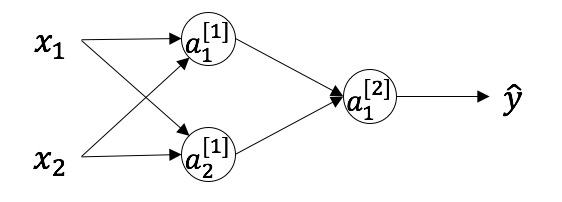
\includegraphics[width=20em]{figures/randomly-init}
    \caption{A shallow neural network with all weights and parameters initialized to 0}
    \label{fig:randomly-init}
\end{figure}

As the Figure~\ref{fig:randomly-init} shows, there is a shallow neural network with two input
features, two hidden units and one output unit. Then we initialized all the weights and parameters
to zero:
\begin{IEEEeqnarray*}{rCl}
    \Matrix{W^{[1]}} = \left[\begin{array}{cc} 0 & 0 \\ 0 & 0 \end{array}\right] \qquad
    \Vector{b^{[1]}} = \left[\begin{array}{c} 0 \\ 0 \end{array}\right] \qquad
    \Matrix{W^{[2]}} = \left[\begin{array}{cc} 0 & 0 \end{array}\right] \qquad
    \Vector{b^{[2]}} = [0]
\end{IEEEeqnarray*}

It turns out that initializing the bias terms $\Vector{b}$ to all zero is exactly okay, but
initializing $\Matrix{W}$ to all zero causes a problem. So the problem with this formalization is
that for any example you give it, you'll have that $a_1^{[1]} = a_2^{[2]}$, and then when you
compute backpropagation, it turns out that $\text{d}z_1^{[1]} = \text{d}z_2^{[2]}$.

If we initialize the neural network this way, the hidden unit $a_1^{[1]}$ and $a_2^{[1]}$ will be
completely identical (symmetric). It turns out that after every single iteration of training, the
two hidden units are still computing exactly the same function, both units have the same
influence on the output unit. The $\text{d}\Matrix{W^{[1]}}$ and $\Matrix{W^{[1]}}$ will looks like
as the following:
\begin{IEEEeqnarray*}{rCl}
    \text{d}\Matrix{W} = \left[\begin{array}{cc} u & v \\ u & v \end{array}\right] \qquad
    \Matrix{W^{[1]}} = \Matrix{W^{[1]}} - \alpha \text{d}\Matrix{W} \qquad
    \Matrix{W^{[1]}} = \left[\begin{array}{cc} r & s \\ r & s \end{array}\right]
\end{IEEEeqnarray*}

So in this case there is really no point to have more than one hidden unit, because all units are
computing the same thing. However, that's not helpful, because you want different units compute
different functions. The solution is to initialize the weights randomly:
\begin{IEEEeqnarray*}{rCl}
    \Matrix{W^{[1]}} = \text{np.random.randn((2, 2)) * 0.01} \qquad
    \Vector{b^{[1]}} = \text{np.zero((2, 1))}
\end{IEEEeqnarray*}
\begin{IEEEeqnarray*}{rCl}
    \Matrix{W^{[2]}} = \text{np.random.randn((1, 2)) * 0.01} \qquad
    \Vector{b^{[2]}} = \text{np.zero((1, 1))}
\end{IEEEeqnarray*}

Why we multiply a factor 0.01? That's because when we use the sigmoid or tanh activation function,
if the weight is large, then the value input to the activation function will be large, so in that
case the slope of the gradient is small and the gradient descent will be very slow.

\section{Deep Neural Networks}
\subsection{Deep $L$-layer neural network}
\paragraph{What is a deep neural network?}
As Figure~\ref{fig:nn-examples} shows, logistic regresssion can be
seen as one layer neural network. When we count the layers of the neural network, we don't count
the input layer. Technically logistic regression is a quite shallow neural network, but over the
last several years, the AI and machine learning community has realized that there are functions
that very deep neural networks can learn while shallower are unable to.
\begin{figure}[htb]
    \centering
    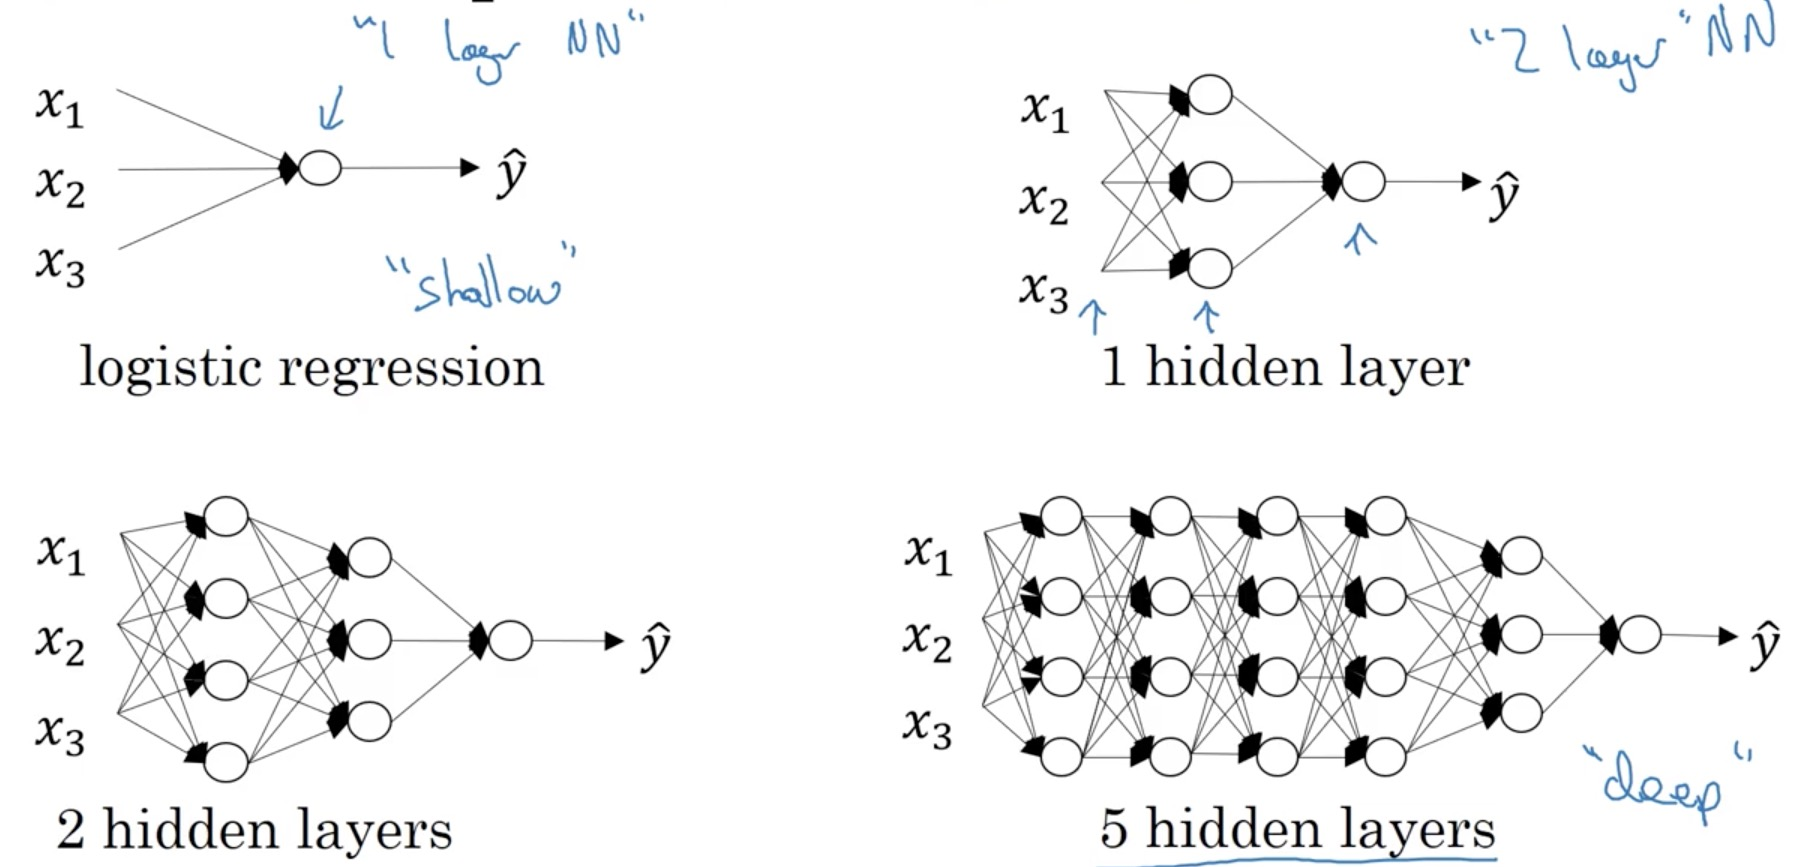
\includegraphics[width=45em]{figures/nn-examples}
    \caption{Examples of neural networks}
    \label{fig:nn-examples}
\end{figure}

\paragraph{Deep neural network notation}
\begin{figure}[htb]
    \centering
    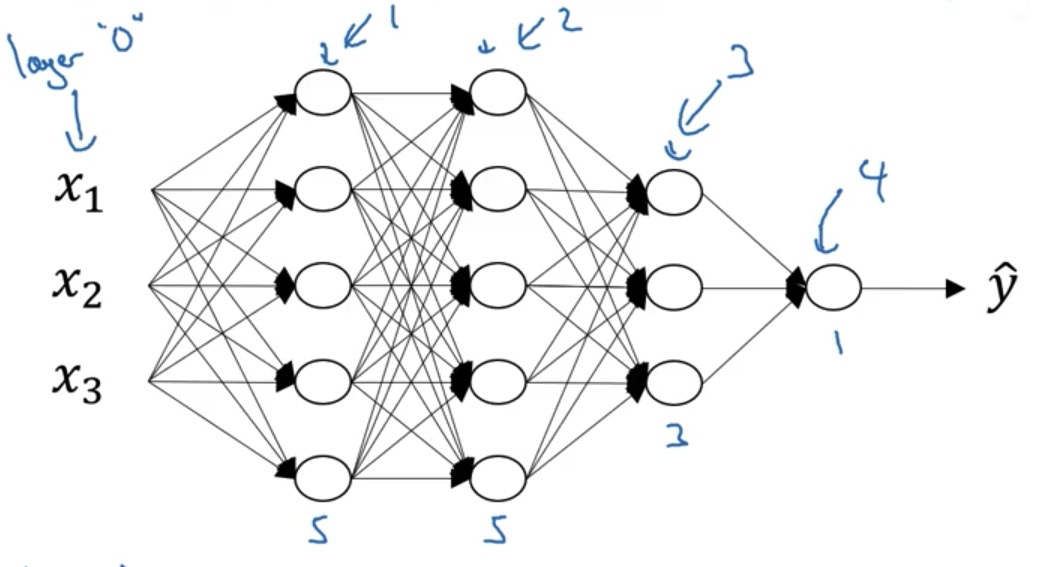
\includegraphics[width=30em]{figures/four-layer-nn}
    \caption{A 4-layer neural network}
    \label{fig:four-layer-nn}
\end{figure}

Figure~\ref{fig:four-layer-nn} shows a 4-layer neural network, with the input layer as ``layer 0'',
three hidden layers ``layer 1'', ``layer 2'' and ``layer 3'', the output layer as ``layer 4''.
Some notations should be remembered as the following:
\begin{description}
    \item[$L$:] \# layers. In Figure~\ref{fig:four-layer-nn}, $L = 4$.
    \item[$n^{[l]}$:] \# units in layer $l$. In this case, $n^{[1]} = 5, n^{[2]} = 5, n^{[3]} = 3,
    n^{[4]} = n^{[L]} = 1, n^{[0]} = n_x = 3$.
    \item[$\Vector{a}^{[l]}$:] activations in layer $l$. In propagation, we will implement
    $\Vector{a}^{[l]} = g^{[1]}(\Vector{z}^{[l]})$. For single example,
    $\Vector{a^{[0]}} = \Vector{x}$, $\Vector{a}^{[L]} = \Vector{\hat{y}}$
    \item[$\Matrix{W}^{[l]}$:] weights for $\Vector{z}^{[l]}$.
\end{description}

\subsection{Forward Propagation in a Deep Network}
We still look at the Figure~\ref{fig:four-layer-nn}, see the forward propagation in this neural
network.
\pagebreak[6]

For every single example,
\begin{IEEEeqnarray*}{rCl}
    \Vector{z^{[1]}} = \Matrix{W^{[1]}} \Vector{a^{[0]}} + \Vector{b^{[1]}}
    = \Matrix{W^{[1]}} \Vector{x} + \Vector{b^{[1]}}
\end{IEEEeqnarray*}
\begin{IEEEeqnarray*}{rCl}
    \Vector{a^{[1]}} = g^{[1]}(\Vector{z^{[1]}})
\end{IEEEeqnarray*}
\begin{IEEEeqnarray*}{rCl}
    \Vector{z^{[2]}} = \Matrix{W^{[2]}} \Vector{a^{[1]}} + \Vector{b^{[2]}}
\end{IEEEeqnarray*}
\begin{IEEEeqnarray*}{rCl}
    \Vector{a^{[2]}} = g^{[2]}(\Vector{z^{[2]}})
\end{IEEEeqnarray*}
\begin{IEEEeqnarray*}{rCl}
    \Vector{z^{[3]}} = \Matrix{W^{[3]}} \Vector{a^{[2]}} + \Vector{b^{[3]}}
\end{IEEEeqnarray*}
\begin{IEEEeqnarray*}{rCl}
    \Vector{a^{[3]}} = g^{[3]}(\Vector{z^{[3]}})
\end{IEEEeqnarray*}
\begin{IEEEeqnarray*}{rCl}
    \Vector{z^{[4]}} = \Matrix{W^{[4]}} \Vector{a^{[3]}} + \Vector{b^{[4]}}
\end{IEEEeqnarray*}
\begin{IEEEeqnarray*}{rCl}
    \Vector{a^{[4]}} = g^{[4]}(\Vector{z^{[4]}}) = \Vector{\hat{y}}
\end{IEEEeqnarray*}

Then we can get the general rule for forward propagation:
\begin{IEEEeqnarray*}{rCl}
    \Vector{z}^{[l]} = \Matrix{W}^{[l]} \Vector{a}^{[l-1]} + \Vector{b}^{[l]}
\end{IEEEeqnarray*}
\begin{IEEEeqnarray*}{rCl}
    \Vector{a}^{[l]} = g^{[l]}(\Vector{z^{[l]}})
\end{IEEEeqnarray*}

For the whole training set, in a vectorized way:
\begin{multicols}{2}
    \begin{IEEEeqnarray*}{rCl}
        \Matrix{Z^{[1]}} = \Matrix{W^{[1]}} \Matrix{A^{[0]}}  + \Vector{b^{[1]}}
        = \Matrix{W^{[1]}} \Matrix{X}  + \Vector{b^{[1]}}
    \end{IEEEeqnarray*}
    \begin{IEEEeqnarray*}{rCl}
        \Matrix{A^{[1]}} = g^{[1]}(\Matrix{Z^{[1]}})
    \end{IEEEeqnarray*}
    \begin{IEEEeqnarray*}{rCl}
        \Matrix{Z^{[2]}} = \Matrix{W^{[2]}} \Matrix{A^{[1]}}  + \Vector{b^{[2]}}
    \end{IEEEeqnarray*}
    \begin{IEEEeqnarray*}{rCl}
        \Matrix{A^{[2]}} = g^{[2]}(\Matrix{Z^{[2]}})
    \end{IEEEeqnarray*}
    \begin{IEEEeqnarray*}{rCl}
        \Matrix{Z^{[3]}} = \Matrix{W^{[3]}} \Matrix{A^{[2]}}  + \Vector{b^{[3]}}
    \end{IEEEeqnarray*}
    \begin{IEEEeqnarray*}{rCl}
        \Matrix{A^{[3]}} = g^{[3]}(\Matrix{Z^{[3]}})
    \end{IEEEeqnarray*}
    \begin{IEEEeqnarray*}{rCl}
        \Matrix{Z^{[4]}} = \Matrix{W^{[4]}} \Matrix{A^{[3]}}  + \Vector{b^{[4]}}
    \end{IEEEeqnarray*}
    \begin{IEEEeqnarray*}{rCl}
        \Matrix{A^{[4]}} = g^{[4]}(\Matrix{Z^{[4]}}) = \Matrix{\hat{Y}}
    \end{IEEEeqnarray*}
    \columnbreak

    We can put the left into a explicit for-loop:
    \begin{algorithm}[H]
        \For{$l = 1$ \KwTo 4}{
        \begin{IEEEeqnarray*}{rCl}
            \Matrix{Z^{[l]}} = \Matrix{W^{[l]}} \Matrix{A^{[l-1]}}  + \Vector{b^{[l]}}
        \end{IEEEeqnarray*}
        \begin{IEEEeqnarray*}{rCl}
            \Matrix{A^{[l]}} = g^{[l]}(\Matrix{Z^{[l]}})
        \end{IEEEeqnarray*}
        }
    \end{algorithm}
\end{multicols}

\subsection{Getting your matrix dimensions right}
\begin{figure}[htb]
    \centering
    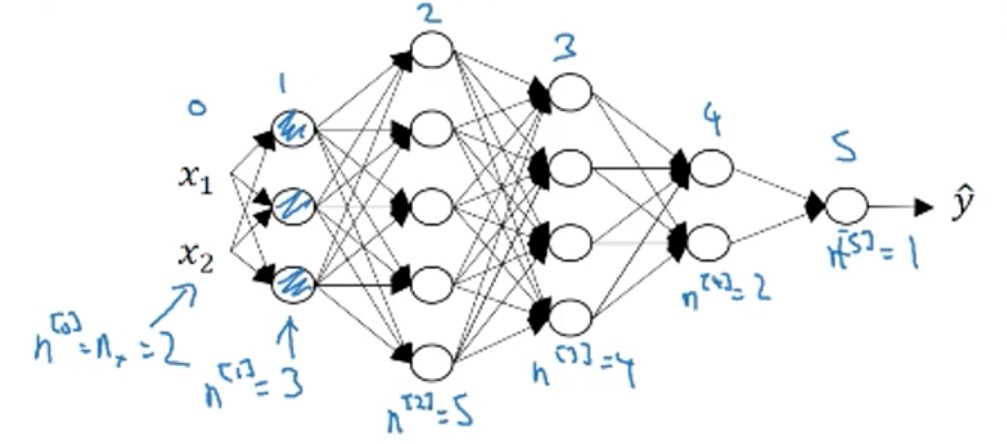
\includegraphics[width=35em]{figures/five-layer-nn}
    \caption{A 5-layer neural network}
    \label{fig:five-layer-nn}
\end{figure}

In Figure~\ref{fig:five-layer-nn}, there is a five-layer neural network, with $n^{[0]} = n_x = 2$,
$n^{[1]} = 3$, $n^{[2]} = 5$, $n^{[3]} = 4$, $n^{[4]} = 2$ and $n^{[5]} = 1$. The checking of the
matrix dimensions can be seen as following.
\paragraph{For every single example}
\begin{IEEEeqnarray*}{rCl}
    \underbrace{\Vector{z^{[1]}}}_{(n^{[1]}, 1) = (3, 1)}
    = \underbrace{\underbrace{\Matrix{W^{[1]}}}_{(n^{[1]}, n^{[0]}) = (3, 2)}
    \underbrace{\Vector{x}}_{(n^{[0]}, 1) = (2, 1)}}_{(3, 1)}
    + \underbrace{\Vector{b^{[1]}}}_{(n^{[1]}, 1) = (3, 1)}
\end{IEEEeqnarray*}
\begin{IEEEeqnarray*}{rCl}
    \underbrace{\Matrix{Z^{[2]}}}_{(n^{[2]}, 1) = (5, 1)}
    = \underbrace{\Matrix{W^{[2]}}}_{(n^{[2]}, n^{[1]}) = (5, 3)}
    \underbrace{\Vector{a^{[1]}}}_{(3, 1)} + \underbrace{\Vector{b^{[2]}}}_{(n^{[2]}, 1) = (5, 1)}
\end{IEEEeqnarray*}
\begin{IEEEeqnarray*}{rCl}
    \ldots\ldots
\end{IEEEeqnarray*}
\begin{IEEEeqnarray*}{rCl}
    \Matrix{W^{[3]}} : (n^{[3]}, n^{[2]}) = (4, 5) \qquad
    \Matrix{W^{[4]}} : (n^{[4]}, n^{[3]}) = (2, 4) \qquad
    \Matrix{W^{[5]}} : (n^{[5]}, n^{[4]}) = (1, 2)
\end{IEEEeqnarray*}
\begin{IEEEeqnarray*}{rCl}
    \Vector{z^{[3]}}, \Vector{a^{[3]}}, \Vector{b^{[3]}} : (n^{[3]}, 1) = (4, 1) \qquad
    \Vector{z^{[4]}}, \Vector{a^{[4]}}, \Vector{b^{[4]}} : (n^{[4]}, 1) = (3, 1) \qquad
    \Vector{z^{[5]}}, \Vector{a^{[5]}}, \Vector{b^{[5]}} : (n^{[5]}, 1) = (1, 1)
\end{IEEEeqnarray*}

The general formula to check is that when you're implementing the matrix $\Matrix{W}$ for layer
$l$, the dimension of that matrix will be $(n^{[l]}, n^{[l-1]})$. And if you're implementing the
back-propagation, the matrix d$\Matrix{W}$ will have the same dimension with $\Matrix{W}$, the
vector d$\Vector{b}$ will have the same dimension with $\Vector{b}$. So for each single example,
the formula is:
\begin{IEEEeqnarray*}{rCl}
    \Matrix{W}^{[l]} : (n^{[l]}, n^{[l-1]}) \qquad \text{d}\Matrix{W}^{[l]} : (n^{[l]}, n^{[l-1]})
\end{IEEEeqnarray*}
\begin{IEEEeqnarray*}{rCl}
    \Vector{z}^{[l]}, \Vector{a}^{[l]}, \Vector{b}^{[l]} : (n^{[l]}, 1) \qquad
    \text{d}\Vector{z}^{[l]}, \text{d}\Vector{a}^{[l]}, \text{d}\Vector{b}^{[l]} : (n^{[l]}, 1)
\end{IEEEeqnarray*}

\paragraph{Vectorized implementation}
\begin{IEEEeqnarray*}{rCl}
    \underbrace{\Matrix{Z^{[1]}}}_{(n^{[1]}, m)}
    = \underbrace{\underbrace{\Matrix{W^{[1]}}}_{(n^{[1]}, n^{[0]})}
    \underbrace{\Matrix{X}}_{(n^{[0]}, m)}}_{(n^{[1]}, m)}
    + \underbrace{\Vector{b^{[1]}}}_{(n^{[1]}, 1) \rightarrow (n^{[1]}, m)}
\end{IEEEeqnarray*}
\begin{IEEEeqnarray*}{rCl}
    \ldots\ldots
\end{IEEEeqnarray*}

Stack all $m$ training examples together, then we can get the vectorized version of the formula:
\begin{IEEEeqnarray*}{rCl}
    \Matrix{W}^{[l]} : (n^{[l]}, n^{[l-1]}) \qquad \text{d}\Matrix{W}^{[l]} : (n^{[l]}, n^{[l-1]})
\end{IEEEeqnarray*}
\begin{IEEEeqnarray*}{rCl}
    \Vector{b}^{[l]} : (n^{[l]}, 1) \qquad
    \text{d}\Vector{b}^{[l]} : (n^{[l]}, 1)
\end{IEEEeqnarray*}
\begin{IEEEeqnarray*}{rCl}
    \Matrix{Z}^{[l]}, \Matrix{A}^{[l]} : (n^{[l]}, m) \qquad
    \text{d}\Matrix{Z}^{[l]}, \text{d}\Matrix{A}^{[l]} : (n^{[l]}, m)
\end{IEEEeqnarray*}

\subsection{Why deep representations?}
\subsubsection{Intuition about deep representation}
\begin{figure}[htb]
    \centering
    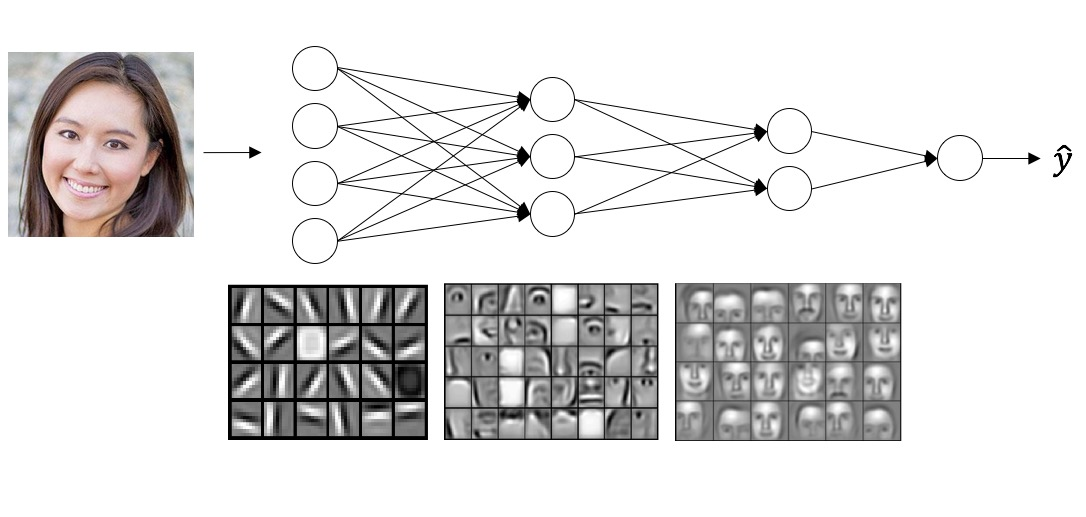
\includegraphics[width=40em]{figures/dnn-intuition}
    \caption{Intuition about deep representation}
    \label{fig:dnn-intuition}
\end{figure}

Like Figure~\ref{fig:dnn-intuition} shows, if you are building a system for face recognition or
face detectioin, here's what a deep neural network could be doing. Perhaps you input a picture of
a face then the first layer of the neural network you can think of as maybe being a feature
detector or an edge detector.

In this example, there are about 20 units in the hidden layer. So the 20 hidden units are
visualized by these little square boxes. So for example, this little visualization in the first
hidden layer represents the hidden unit is trying to figure out where the edges of that orientation
in the image.

Now, let's think about where the edges in this picture by grouping together pixels to form edges.
It can then detect the edges and group edges together to form parts of the faces. So for example,
you might have a neuron trying to see if it's finding an eye, or a different neuron trying to find
that part of the nose. So by putting together lots of edges, it can start to detect different parts
of faces.

Finally, by putting together different parts of faces, like an eye or a nose or an ear or a chin,
it can try to recognize or detect different types of faces.

So intuitively, you can think of the earlier layers of the neural network as detecting simple
functions, like edges. And then composing them together in the later layers of a neural network so
that it can learn more and more complex functions. These visualizations will make more sense when
we talk about convolutional nets.

\subsubsection{Circuit theory and deep learning}
Informally: There are functions you can compute with a ``small'' (hidden units) $L$-layer deep neural
network that shallower networks require exponentially more hidden units to compute.

\begin{figure}[htb]
    \centering
    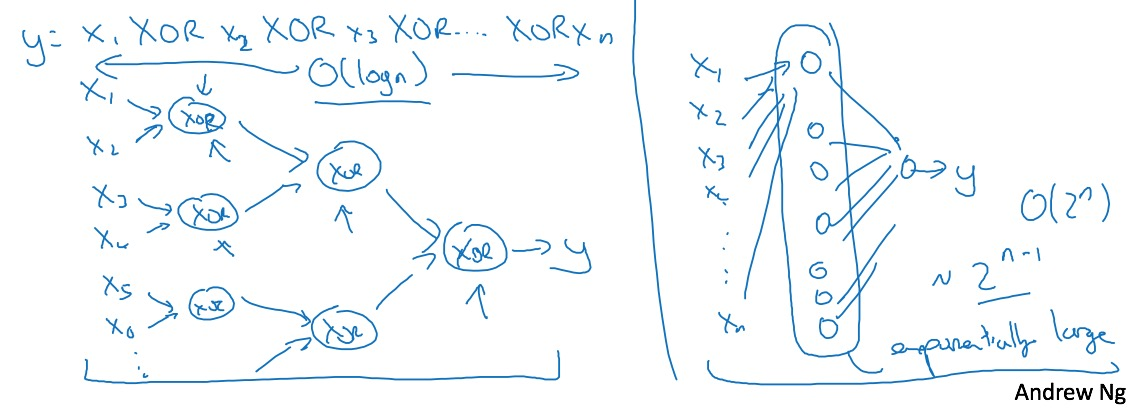
\includegraphics[width=40em]{figures/circuit-theory-and-dl}
    \caption{Use deep neural networks and shallower neural networks to implement the XOR of $n$
    input. For deep neural network (the left one), to compute the XOR, the depth of the network
    will be on the order of $O(\log n)$, so the number of nodes, or the number of circuit
    components or the number of gates in this neural network is not that large. But if you are
    forced to compute the function with just one hidden layer, then in order to get the parity
    of XOR to compute this XOR function, the size of this hidden layer will need to be exponentially
    large ($2^{n-1}$), because essentially you need to exhaustively enumerate all 2 to the $n$ possible
    configurations.}
    \label{circuit-theory-and-dl}
\end{figure}

\subsection{Building blocks of deep neural networks}
For the layer $l$ in the deep neural network:
\begin{description}
    \item[Parameters:] $\Matrix{W}^{[1]}$, $\Vector{b}^{[l]}$.
    \item[Forward:] input: $\Vector{a}^{[l-1]}$; output: $\Vector{a}^{[l]}$;
    cache ($\Vector{z^{[l-1]}}$). \\
    $\Vector{z}^{[l]} = \Matrix{W}^{[l]} \Vector{a}^{[l-1]} + \Vector{b}^{[l]}$ \\
    $\Vector{a}^{[l]} = g^{[l]}(\Vector{z}^{[l]})$ \\
    Vectorized version: \\
    $\Matrix{Z}^{[l]} = \Matrix{W}^{[l]} \Matrix{A}^{[l-1]} + \Vector{b}^{[l]}$ \\
    $\Matrix{A}^{[l]} = g^{[l]}(\Matrix{Z}^{[l]})$
    \item[Backward:] input: d$\Vector{a}^{[l]}$ (get from cache ($\Vector{z^{[l-1]}}$));
    output: d$\Vector{a}^{[l-1]}$, d$\Matrix{W}^{[l]}$, d$\Vector{b}^{[l]}$; \\
    d$\Vector{z}^{[l]} = \text{d}\Vector{a}^{[l]} * {g^{[l]}}'(\Vector{z}^{[l]})$ \\
    d$\Matrix{W}^{[l]} = \text{d}\Vector{z}^{[l]} \Vector{a}^{[l-1]}$ \\
    d$\Vector{b}^{[l]} = \text{d}\Vector{z}^{[l]}$ \\
    d$\Vector{a}^{[l-1]} = {\Matrix{W}^{[l]}}^T \text{d}\Vector{z}^{[l]}$ \\
    Vectorized version: \\
    d$\Matrix{Z}^{[l]} = \text{d}\Matrix{A}^{[l]} * {g^{[l]}}'(\Matrix{Z}^{[l]})$ \\
    d$\Matrix{W}^{[l]} = \frac{1}{m} \text{d}\Matrix{Z}^{[l]} {\Matrix{A}^{[l-1]}}^T$ \\
    d$\Vector{b}^{[l]}
        = \frac{1}{m} \text{np.sum(d} \Matrix{Z}^{[l]} \text{, axis=1, keepdims=True)}$ \\
    d$\Matrix{A}^{[l-1]} = {\Matrix{W}^{[l]}}^T \text{d}\Matrix{Z}^{[l]}$
\end{description}

The process above can be concluded as a block in Figure~\ref{fig:dnn-block}.

\begin{figure}[htb]
    \centering
    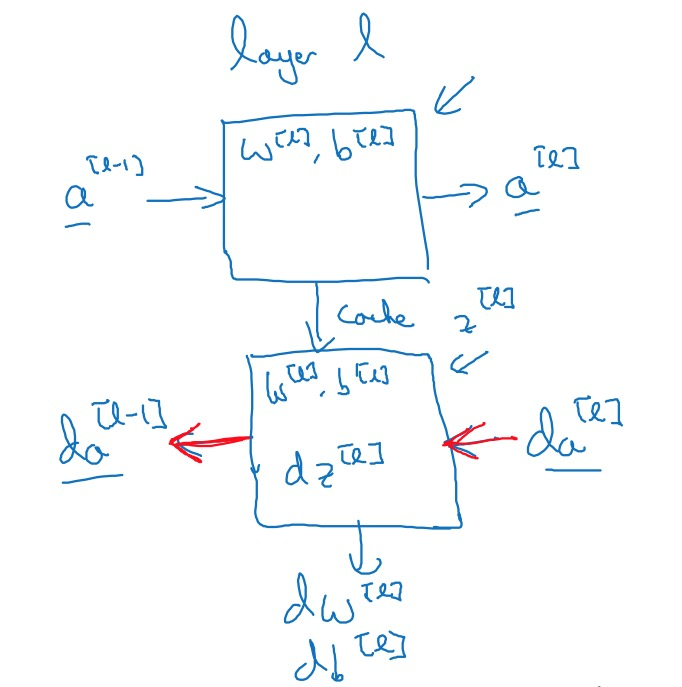
\includegraphics[width=25em]{figures/dnn-block}
    \caption{A block of forward and backward process in a deep Neural network}
    \label{fig:dnn-block}
\end{figure}

\subsection{Parameters vs Hyperparameters}
\subsubsection{What are hyperparameters?}
\begin{description}
    \item[Paramters:] $\Matrix{W^{[1]}}$, $\Vector{b^{[1]}}$, $\Matrix{W^{[2]}}$,
    $\Vector{b^{[2]}}$, $\Matrix{W^{[3]}}$, $\Vector{b^{[3]}}$ \ldots
    \item[Hyperparameters:] learning rate $\alpha$; \# iterations; \# hidden layer $L$;
    \# hidden units $n^{[1]}$, $n^{[2]}$, \ldots; choice of activation function.
\end{description}

Hyperparamters are parameters that control parameters $\Matrix{W}$ and $\Vector{b}$. In later
course, we will learn other hyperparameters such as momentum, mini-batch size and regularization
parameters.

\subsubsection{Applied deep learning is a very empirical process}
Applied deep learning today is a very empirical process. For example, in
Figure~\ref{fig:hyperparameters} you have an idea that set $\alpha = 0.01$, then you implement it,
try out and see how that works, and then based on the outcome you might say you know that I have
changed my mind, then you do the process again to try $\alpha = 0.05$. You might plot the cost $J$
of the number of iterations to see which is the best learning rate.

\begin{figure}[htb]
    \centering
    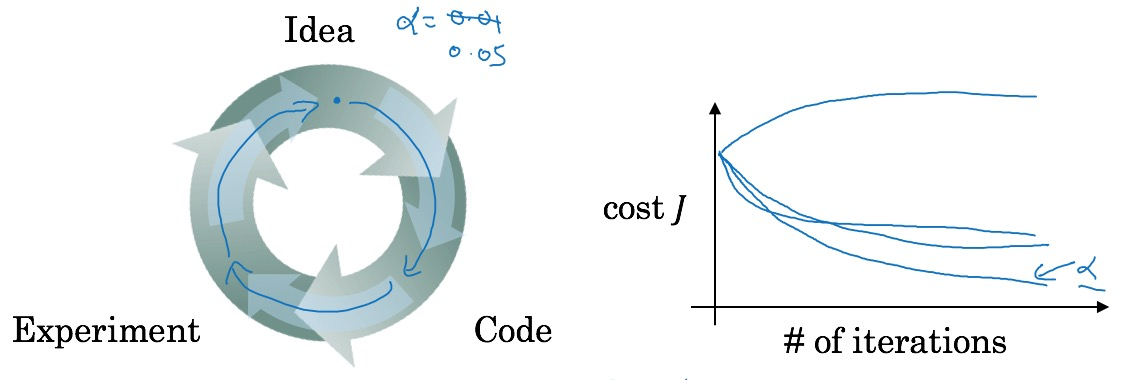
\includegraphics[width=40em]{figures/hyperparameters}
    \caption{The process of try different hyperparamters in a deep Neural network}
    \label{fig:hyperparameters}
\end{figure}

The `empirical process' in the title means that you have to try a lit if things and see what works.
When starting on a new problem, just try out a range of values and see what works. In the next
course, we'll see some systematic ways for trying out a range of values of hyperprameters.

Secondly, if you're working on one application for a long time, maybe you're working on online
advertising as you make progress on the problem is quite possible there the best value for the
learning rate, a number of hidden units and so on might change, even if you tune your system to
the best value of hyperparameters today, it's possible that you find taht the best value might
change year from now.


\end{document}
